\documentclass[]{article}
\usepackage{graphicx}
\usepackage[svgnames]{xcolor} 
\usepackage{fancyhdr}

\usepackage{hyperref}
\usepackage{enumitem}
\usepackage[many]{tcolorbox}
\usepackage{listings }
\usepackage[a4paper, total={6in, 8in}]{geometry}
\usepackage{afterpage}
\usepackage{amssymb}
\usepackage{pdflscape}
\usepackage{textcomp}
\usepackage{xecolor}
\usepackage{rotating}
\usepackage[Kashida]{xepersian}
\usepackage[T1]{fontenc}
\usepackage{tikz}
\usepackage[utf8]{inputenc}
\usepackage{PTSerif} 
\usepackage{seqsplit}
\usepackage[edges]{forest}

\usepackage{listings}
\usepackage{xcolor}
 
\definecolor{codegreen}{rgb}{0,0.6,0}
\definecolor{codegray}{rgb}{0.5,0.5,0.5}
\definecolor{codepurple}{rgb}{0.58,0,0.82}
\definecolor{backcolour}{rgb}{0.95,0.95,0.92}
 
\NewDocumentCommand{\codeword}{v}{
\texttt{\textcolor{blue}{#1}}
}
\lstset{language=java,keywordstyle={\bfseries \color{blue}}}

\lstdefinestyle{mystyle}{
    backgroundcolor=\color{backcolour},   
    commentstyle=\color{codegreen},
    keywordstyle=\color{magenta},
    numberstyle=\tiny\color{codegray},
    stringstyle=\color{codepurple},
    basicstyle=\ttfamily\normalsize,
    breakatwhitespace=false,         
    breaklines=true,                 
    captionpos=b,                    
    keepspaces=true,                 
    numbers=left,                    
    numbersep=5pt,                  
    showspaces=false,                
    showstringspaces=false,
    showtabs=false,                  
    tabsize=2
}

\lstset{style=mystyle}

\settextfont[BoldFont={XB Zar bold.ttf}]{XB Zar.ttf}




\newcommand{\inputsample}[1]{
    ~\\
    \textbf{ورودی نمونه}
    ~\\
    \begin{tcolorbox}[breakable,boxrule=0pt]
        \begin{latin}
            \large{
                #1
            }
        \end{latin}
    \end{tcolorbox}
}

\newcommand{\outputsample}[1]{
    ~\\
    \textbf{خروجی نمونه}

    \begin{tcolorbox}[breakable,boxrule=0pt]
        \begin{latin}
            \large{
                #1
            }
        \end{latin}
    \end{tcolorbox}
}

\newenvironment{changemargin}[2]{%
\begin{list}{}{%
\setlength{\topsep}{0pt}%
\setlength{\leftmargin}{#1}%
\setlength{\rightmargin}{#2}%
\setlength{\listparindent}{\parindent}%
\setlength{\itemindent}{\parindent}%
\setlength{\parsep}{\parskip}%
}%
\item[]}{\end{list}}
%%%%%باکس های طراحی شده برای پاسخ نامه ، میتوانید پاسخ را درون باکس قراردهید
\newtcolorbox[auto counter]{solutionbox}{
freelance,
colback=white,
frame code={},
interior titled code={
  \fill[rounded corners=8pt,orange!30]
    (title.south west) --
    (title.south) -- 
    ([yshift=20pt]title.south) --
    ([yshift=20pt,xshift=4cm]title.south) --
    ([xshift=4cm]title.south) --
    (title.south east) {[sharp corners] --
    ([yshift=-6pt]title.south east) -- 
    ([yshift=-6pt]title.south west) } -- cycle;
  \draw[rounded corners=8pt,gray,line width=1pt]
    (title.west|-frame.south west) --
    (title.south west) --
    (title.south) -- 
    ([yshift=20pt]title.south) --
    ([yshift=20pt,xshift=4cm]title.south) --
    ([xshift=4cm]title.south) --
    (title.south east) --
    (title.east|-frame.south east) --
    cycle;
  \node at ([xshift=2cm,yshift=4pt,anchor=south]title.south) 
    {\Large \textbf{پاسخ}};  
  },
title={\mbox{}},
top=12pt,
fontupper=\sffamily\Large,
oversize=0.5cm,
before={\vskip24pt\par\noindent},
after={\par\vskip12pt}
}
\newtcolorbox[auto counter]{solutionboxC}{
freelance,
colback=white,
frame code={},
interior titled code={
  \fill[rounded corners=8pt,orange!30]
    (title.south west) --
    (title.south) -- 
    ([yshift=20pt]title.south) --
    ([yshift=20pt,xshift=4cm]title.south) --
    ([xshift=4cm]title.south) --
    (title.south east) {[sharp corners] --
    ([yshift=-6pt]title.south east) -- 
    ([yshift=-6pt]title.south west) } -- cycle;
  \draw[rounded corners=8pt,gray,line width=1pt]
    (title.west|-frame.south west) --
    (title.south west) --
    (title.south) -- 
    ([yshift=20pt]title.south) --
    ([yshift=20pt,xshift=4cm]title.south) --
    ([xshift=4cm]title.south) --
    (title.south east) --
    (title.east|-frame.south east) --
    cycle;
  \node at ([xshift=2cm,yshift=4pt,anchor=south]title.south) 
    {\Large \textbf{ پاسخ ادامه}};  
  },
title={\mbox{}},
top=12pt,
fontupper=\sffamily\Large,
oversize=0.5cm,
before={\vskip24pt\par\noindent},
after={\par\vskip12pt}
}

\definecolor{foldercolor}{RGB}{124,166,198}

\tikzset{pics/folder/.style={code={%
    \node[inner sep=0pt, minimum size=#1](-foldericon){};
    \node[folder style, inner sep=0pt, minimum width=0.3*#1, minimum height=0.6*#1, above right, xshift=0.05*#1] at (-foldericon.west){};
    \node[folder style, inner sep=0pt, minimum size=#1] at (-foldericon.center){};}
    },
    pics/folder/.default={20pt},
    folder style/.style={draw=foldercolor!80!black,top color=foldercolor!40,bottom color=foldercolor}
}

\forestset{is file/.style={edge path'/.expanded={%
        ([xshift=\forestregister{folder indent}]!u.parent anchor) |- (.child anchor)},
        inner sep=1pt},
    this folder size/.style={edge path'/.expanded={%
        ([xshift=\forestregister{folder indent}]!u.parent anchor) |- (.child anchor) pic[solid]{folder=#1}}, inner xsep=0.6*#1},
    folder tree indent/.style={before computing xy={l=#1}},
    folder icons/.style={folder, this folder size=#1, folder tree indent=3*#1},
    folder icons/.default={12pt},
}

\begin{document}


%%% title pages
\begin{titlepage}
\begin{center}
        
\vspace*{0.7cm}


\includegraphics[width=0.4\textwidth]{sharif1.png}\\
\vspace{0.5cm}
\textbf{ \Huge{\emph درس برنامه‌سازی پیشرفته} }\\
\vspace{0.5cm}
\textbf{ \Large{ تمرین دوم} }
\vspace{0.2cm}
       
 
      \large \textbf{دانشکده مهندسی کامپیوتر}\\\vspace{0.2cm}
    \large   دانشگاه صنعتی شریف\\\vspace{0.2cm}
       \large   ﻧﯿﻢ سال دوم 99-98 \\\vspace{0.2cm}
      \noindent\rule[1ex]{\linewidth}{1pt}
اساتید:\\
    \textbf{{مهدی مصطفی‌زاده، ایمان عیسی‌زاده، امیر ملک‌زاده، علی چکاه}}

    \vspace{0.20cm}
    مبحث:\\
    \textbf{{برنامه نویسی شی‌‌گرا}}

    \vspace{0.20cm}

   مهلت ارسال:\\
    \textbf{{12 فروردین}}\\
    \textbf{{ساعت 23:59:59}}

    \vspace{0.15cm}
ویراستار فنی:\\
    \textbf{{امیرمهدی نامجو و صابر ظفرپور}}
\end{center}
\end{titlepage}
%%% title pages


%%% header of pages
\newpage
\pagestyle{fancy}
\fancyhf{}
\fancyfoot{}
\cfoot{\thepage}
\chead{برنامه نویسی شی‌‌گرا}
\rhead{
\includegraphics[width=0.1\textwidth]{sharif.png}}
\lhead{تمرین ۲ برنامه‌سازی پیشرفته}
%%% header of pages

\KashidaOff


 \Large \textbf{\\\\
به موارد زیر توجه کنید:}

\begin{itemize}[label=$\ast$]
\item  به ازای هر سوال در سامانه کوئرا بخش جداگانه ای برای آپلود شما وجود دارد. شما باید تمامی فایل‌های کلاس‌هایی که با فرمت .java نوشته‌اید را در قالب فشرده با فرمت .zip در آورده و در سامانه کوئرا آپلود کنید. توجه کنید که حتما فایل حاوی کلاسی که تابع
\begin{latin}
\codeword{public static void main(string[] args)}
\end{latin}
در آن قرار دارد و اجرای برنامه از آن جا شروع می‌شود، باید بدون قرار گرفتن در هیچ پوشه‌ای درون فایل zip قرار بگیرد و نام آن هم Main.java باشد. امکان پوشه بندی و ایجاد package های مختلف برای سایر فایل‌ها امکان پذیر است. به عنوان نمونه می‌توانید به ساختار قابل قبولی و درستی که در زیر رسم شده است، توجه کنید. توجه کنید که پوشه src که فایل‌ها در آن قرار دارد، نباید در فایل .zip باشد.

\begin{latin}

\begin{forest}
    for tree={font=\sffamily, grow'=0,
    folder indent=.9em, folder icons,
    edge=densely dotted}
    [answer.zip
      [models
          [Model1.java,is file]
          [Model2.java, is file]]
      [views
          [View1.java, is file]]
          [controllers
          [Controller1.java , is file]
          ]
      [Main.java, is file]
      [MyClass.java, is file]
      [MyClass2.java, is file]
    ]
  \end{forest}



\end{latin}



\item ورودی و خروجی شما باید عیناً شبیه به نمونه‌های ورودی و خروجی باشد؛ لذا عبارت‌هایی همچون \lr{"Enter your number"} را قبل از گرفتن ورودی نباید چاپ کنید.
\item پس از ارسال فایل مربوط به هر سوال، سامانه‌ی کوئرا به‌صورت لحظه‌ای برنامه‌ی شما را داوری کرده و نمره‌ی آن سوال را به شما اعلام می‌کند که در صورت کم بودن نمره‌تان، می‌توانید آن را تصحیح کرده و دوباره ارسال کنید.
\item هم‌فکری و هم‌کاری در پاسخ به تمرینات اشکالی ندارد و حتی توصیه نیز می‌شود؛ ولی پاسخ ارسالی شما باید حتما توسط خود شما نوشته شده‌باشد. در صورت هم‌فکری در مورد یک سوال، نام فرد دیگر را به‌صورت کامنت در ابتدای کد هر سوال بنویسید.
\item شما می‌توانید تمامی سوالات و ابهامات خود را در سایت کوئرا در بخش مشخص‌شده برای این تمرین بپرسید.
\item مهلت ارسال تمرین تا ساعت 23:59:59 روز 12 فروردین 1399 است.
\item به‌ازای هر روز تاخیر در ارسال پاسخ هر سوال، 30 درصد از نمره‌ی کسب‌شده‌ی شما در آن سوال کم می‌شود. به عنوان مثال اگر پاسخ یک سوال را با دو روز تاخیر ارسال کنید، فقط 40 درصد از نمره‌ای که برای آن سوال گرفته‌اید برای شما لحاظ خواهد شد.

\item
از آن جا که هدف این تمرین ، آشنایی با مفاهیم شی گرایی است، رعایت این موارد همانند رعایت ‌کلین‌کد اجباری است.

\item
همچنین در سوال اول نیز شما ملزم به رعایت uml داده شده در طراحی خود هستید.

\item

توجه کنید که به ازای هر روز ارسال زودتر هر سوال به شرط کامل بودن و رعایت نکات تمیزی کد و نکات شی گرایی و طراحی براساس uml در سوال یک ، ۵\% نمره اضافه به شما تعلق می‌گیرد. سقف تعداد روز هایی که برای این موضوع محاسبه می‌شود ، 4 است. یعنی در صورت  چهار روز  ارسال زودتر  ۲۰\% نمره اضافه به شما تعلق می‌گیرد.
\end{itemize}




\newpage
\section{ایزی ایزی}
در کتبِ تاریخی متعددی آمده است که در کشور برزیل (از توابع آبادانِ کنونی)، سیستمِ بانکیِ پیشرفته‌ای وجود داشته و مردمِ آنجا (مِن جمله پله‌ی فقید و آقامون رونالدینیو) به داشتنِ چنین سیستمی افتخار می‌کردند.

\begin{center}
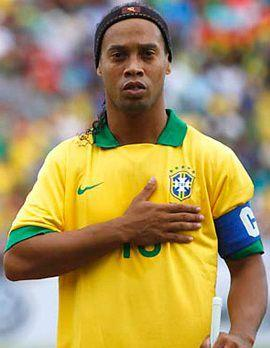
\includegraphics[width=0.4\textwidth]{ronald.jpg}
\end{center}

بر اثر حادثه‌ای تاریخی برزیل از آمریکای جنوبی جدا و به زادگاهِ خود، آبادن برمی‌گردد.

متاسفانه در حین عبور از تنگه‌ی هرمز، بر اثر پهناوریِ بیش از حدِ برزیل، قسمتی از آن به تنگه گیر کرده، شکسته و در آب غرق می‌شود. نکته‌ی بد اینجاست که سیستمِ بانکی برزیل در آن قسمتِ غرق شده قرار داشت و اکنون برزیلِ باقیمانده سیستمِ بانکی ندارد.

در این سوال ما از شما می‌خواهیم تا سیستمِ بانکیِ برزیل را مجددا پیاده سازی کنید. خوشبحتانه نقشه‌ی این سیستمِ بانکی از بین نرفته و در این سوال، شما باید دقیقاً طبق همین نقشه (\textbf{که در اصل به آن UML میگویند}) سیستم بانکی برزیل را مجددا پیاده سازی کنید.

این سیستم بانکی دارای اجزای زیر است:

\textbf{بانک}: در برزیل هر بانک یک \underline{نام مخصوص به خود} دارد و خدماتِ افتتاح حساب و اعطای وام را ارائه می‌کند.


\textbf{مشتری}: هر مشتری \underline{یک اسم مخصوص به خود} دارد و هیچ دو مشتری‌ای اسم یکسان ندارند. \underline{نمره‌ی منفی} ویژگیِ دیگریست که مشتری‌ها دارند. در مورد نمره‌ی منفی در قسمتِ وام خواهید خواند..

هر مشتری در ابتدا مقداری پول در \underline{گاوصندوق خانه اش} دارد. او میتواند یک مقدار از این پول را در هر بانکی در قالبِ یک حساب، سپرده گذاری کند. با تمام شدنِ مدتِ تعیین شده برای حساب، مبلغِ سپرده گذاری شده همراه با سودِ آن به صورت اتوماتیک (!) به گاوصندوقِ مشتری برمیگردد.

اگر مشتری زودتر از مدت تعیین شده برای بازپس گرفتنِ سپرده‌اش به بانک مراجعه کند، تنها مبلغِ اصلی (بدون سود) را دریافت میکند و به گاوصندوقش برمیگرداند.

با پس گرفته شدن پول یک حساب یا به پایان رسیدنِ مدت تعیین شده‌ی حساب، آن حساب از بین میرود.


\textbf{حساب}: سه نوع حساب در بانک های برزیل وجود دارد؛ حساب های \underline{کوتاه‌مدت}، \underline{بلندمدت} و \underline{ویژه}. هر حساب \underline{شماره}، \underline{میزان سپرده‌ی اولیه}، \underline{درصد سود} و \underline{مدتِ تعیین شده‌} دارد. پس از سپری شدن زمانِ تعیین شده، درصد سود به علاوه‌ی 1 شده و  در میزان سپرده‌ی اولیه ضرب می‌شود، سپس به گاوصندوق صاحب حساب بازمی‌گردد.

درصد سود حساب های کوتاه مدت، بلندمدت و ویژه به ترتیب 10\%، 30\% و 50\% است. نوعِ حساب (کوتاه مدت، بلند مدت و ویژه) و مدتِ حساب در هنگامِ ساختن حساب توسط مشتری تعیین میشود.



نکته‌ی دیگر اینکه شماره‌ی هر حسابی که هر مشتری ایجاد می‌کند، یکی بیشتر از تعداد حساب‌هایی میشود که همان مشتری از \underline{بدوِ خلقت تا الان ساخته}؛ برای مثال اگر یک مشتری پنجمین حسابِ خود را ایجاد کند، شماره‌ی آن حساب 5 میشود (یعنی ممکن است در بانکی دو حساب با شماره‌ی یکسان وجود داشته باشد ولی مطمئاً آن دو حساب متعلق به دو نفرِ مختلف هستند.).

\KashidaOn

\textbf{وام}: هر بانک می‌تواند به مشتریان خود وام پرداخت کند. هر وام \underline{درصد سود }و \underline{مقدار} دارد. دو نوع وام داریم: وامِ 6 قسطه و 12 قسطه. بعد از ثبت درخواست، وام به گاوصندوق مشتری وارد میشود. \underline{پرداخت اقساط از انتهای همان واحد زمانی آغاز می‌شود.
}

\KashidaOff
مکانیزم پرداخت اقساط به این صورت است که در هر واحد زمانی یک قسط به مقدار زیر از گاوصندوق مشتری کم می‌شود:

$$\text{مقدار هر قسط}=\frac{\text{مقدار اولیه وام} \times (\text{درصد سود} + \text{1})}{\text{تعداد کل اقساط}}$$

اگر مشتری در گاوصندوق خود به مقدار قسط پول نداشته باشد، هیچ مقداری از گاوصندوق او کم نشده، تعداد اقساطِ باقیمانده‌اش \underline{ثابت می‌ماند} و یک نمره‌ی منفی می‌گیرد.

بدیِ نمره ی منفی این است که اگر مشتری‌ای حداقل پنج نمره‌ منفی داشته باشد دیگر وامی به او تعلق نمی‌گیرد.

به این نکته هم توجه داشته باشید که ترتیبِ کم شدنِ اقساط وام‌ها هم براساس ترتیب به وجود آمدنِ وام‌هاست؛ یعنی مثلاً اگر وامِ x زودتر از وامِ y در ورودی آمده باشد، قسطِ وامِ x زودتر از قسط وامِ y از حسابِ مشتریان کم می‌شود.

عملیات‌هایی که در سیستم بانکی برزیل پشتیبانی می‌شوند به شرح زیر هستند:

\begin{tcolorbox}[boxrule=0pt]
	\begin{latin}
  	  \large{
  	  	Add a customer with name A and N unit initial money.
		}
	\end{latin}
\end{tcolorbox}

افزودن یک مشتری با نامِ A و N واحد پولِ اولیه (که A یک اسمِ یک یا چند بخشی است و N یک عدد طبیعیست).

\hrulefill



\begin{tcolorbox}[boxrule=0pt]
	\begin{latin}
  	  \large{
  	  	Create bank M.
		}
	\end{latin}
\end{tcolorbox}

افزودن بانک با نامِ M (که M یک اسم یک یا چند بخشی است (مثلا “$golabi$” یا “$kaka ~ khan<3$” دو اسمِ مجاز هستند).

\hrulefill



\begin{tcolorbox}[boxrule=0pt]
	\begin{latin}
  	  \large{
  	  	Create a (KOOTAH|BOLAN|VIZHE) account for A in M, with duration T and initial deposit of D.
		}
	\end{latin}
\end{tcolorbox}

افزودن یک حسابِ کوتاه مدت، بلند مدت یا ویژه در بانکِ M با مدت زمانِ T و میزان سپرده‌ی اولیه‌ی D توسط مشتری A.

اگر بانک با نامِ M وجود نداشت، پیغامِ:

\begin{tcolorbox}[boxrule=0pt]
	\begin{latin}
  	  \large{
  	  	In dige banke koodoom keshvarie?
		}
	\end{latin}
\end{tcolorbox}


را چاپ کنید.

اگر مشتری کمتر از D واحد درون گاوصندوق خود پول داشت، پیغامِ

\begin{tcolorbox}[boxrule=0pt]
	\begin{latin}
  	  \large{
  	  	Boro baba pool nadari!
		}
	\end{latin}
\end{tcolorbox}


رو چاپ کنید.

خطاها را به همین ترتیب چک کنید و خروجی دهید

\hrulefill



\begin{tcolorbox}[boxrule=0pt]
	\begin{latin}
  	  \large{
  	  	Give A\textquotesingle s money out of his account number N.
		}
	\end{latin}
\end{tcolorbox}


برداشتن تمام پول شخص A از حسابِ شماره‌ی N.

اگر مشتری حساب با همچین شماره‌ای نداشت، پیغامِ

\begin{tcolorbox}[boxrule=0pt]
	\begin{latin}
  	  \large{
  	  	Chizi zadi?!
		}
	\end{latin}
\end{tcolorbox}

را چاپ کنید.


\hrulefill





\begin{tcolorbox}[boxrule=0pt]
	\begin{latin}
  	  \large{
  	  	Pay a X unit loan with Y\% interest and (6|12) payments from M to A.
		}
	\end{latin}
\end{tcolorbox}

پرداخت یک وام با مقدار X واحد و سودِ Y\% و اقساط 6 یا 12 واحدی از بانکِ M به شخصِ A.

چنانچه بانک با نامِ M وجود نداشته باشد، پیغامِ

\begin{tcolorbox}[boxrule=0pt]
	\begin{latin}
  	  \large{
  	  	Gerefti maro nesfe shabi?
		}
	\end{latin}
\end{tcolorbox}

را چاپ کنید.

چنانچه A حداقل 5 نمره‌ی منفی داشته باشد، پیغامِ:

\begin{tcolorbox}[boxrule=0pt]
	\begin{latin}
  	  \large{
  	  	To yeki kheyli vazet bade!
		}
	\end{latin}
\end{tcolorbox}

را چاپ کنید.




\hrulefill



\begin{tcolorbox}[boxrule=0pt]
	\begin{latin}
  	  \large{
  	  	Pass time by X unit.
		}
	\end{latin}
\end{tcolorbox}

از ابتدای خلقت X واحد میگذرد.

\hrulefill


\begin{tcolorbox}[boxrule=0pt]
	\begin{latin}
  	  \large{
  	  	Print A\textquotesingle s GAVSANDOOGH money.
		}
	\end{latin}
\end{tcolorbox}


میزان پول موجود در گاوصندوق مشتری A را چاپ کنید.


\hrulefill


\begin{tcolorbox}[boxrule=0pt]
	\begin{latin}
  	  \large{
  	  	Print A\textquotesingle s NOMRE MANFI count.
		}
	\end{latin}
\end{tcolorbox}


تعداد نمره های منفی A را چاپ کنید.


\hrulefill

آیا شخصِ A در بانکِ M حساب فعال دارد یا نه؟

\begin{tcolorbox}[boxrule=0pt]
	\begin{latin}
  	  \large{
  	  	Does A have active account in M?
		}
	\end{latin}
\end{tcolorbox}

در صورتی که A در بانکِ M حسابِ فعالی داشته باشد عبارت

\begin{tcolorbox}[boxrule=0pt]
	\begin{latin}
  	  \large{
  	  	yes
		}
	\end{latin}
\end{tcolorbox}

و در غیر این صورت عبارت

\begin{tcolorbox}[boxrule=0pt]
	\begin{latin}
  	  \large{
  	  	no
		}
	\end{latin}
\end{tcolorbox}

را چاپ کنید.

\hrulefill



\begin{tcolorbox}[boxrule=0pt]
	\begin{latin}
  	  \large{
  	  	Base dige, berid khonehatoon.
		}
	\end{latin}
\end{tcolorbox}

انجام عملیات‌های بانکی خاتمه می‌یابد.

\hrulefill

\begin{itemize}

\item
	\underline{پرداخت اقساط وام و کم شدن از مدتِ تعیین شده برای حساب‌ها}، در پایانِ هر واحدِ زمانی اتفاق می‌افتد و سایرِ اعمال از جمله "واریزِ سپرده‌ی حساب‌ها پس از تمام شدنِ مدت حساب"، در ابتدای هر واحدِ زمانی رخ میدهد.
	
\item	
	به نقطه ها و علائم نگارشی آخر دستورات و جملات توجه کنید. در دستورات ورودی و خروجی عیناً همان‌ها آورده می‌شود.

\item	
	تضمین می‌شود تنها خطاهایی که در بالا برای آنها پاسخی آمده رخ میدهند و خطاهای دیگری در دستورات ورودی رخ نمیدهد. ترتیب خطاها را همانگونه که آورده شده چک کنید و خروجی دهید.

\item	
	در هنگام چاپ اعداد در خروجی، آنها را قطع و چاپ کنید؛ مثلا اگر میزان پول موجود در گاوصندوقِ مشتری ،A 34.12 واحد باشد، شما باید عدد 12 را چاپ کنید.

\item

{\xecolor{red} کدی که میزنید حتماً باید براساس UML داده شده در صفحه بعد پیاده سازی شود. این موضوع در تحویل حضوری بررسی خواهد شد. فایل این تصویر نیز به طور جداگانه قرار گرفته است. }	


	
\end{itemize}
\begin{landscape}
\newpage
\begin{changemargin}{2cm}{-4.5cm}
\thispagestyle{empty}
\begin{center}
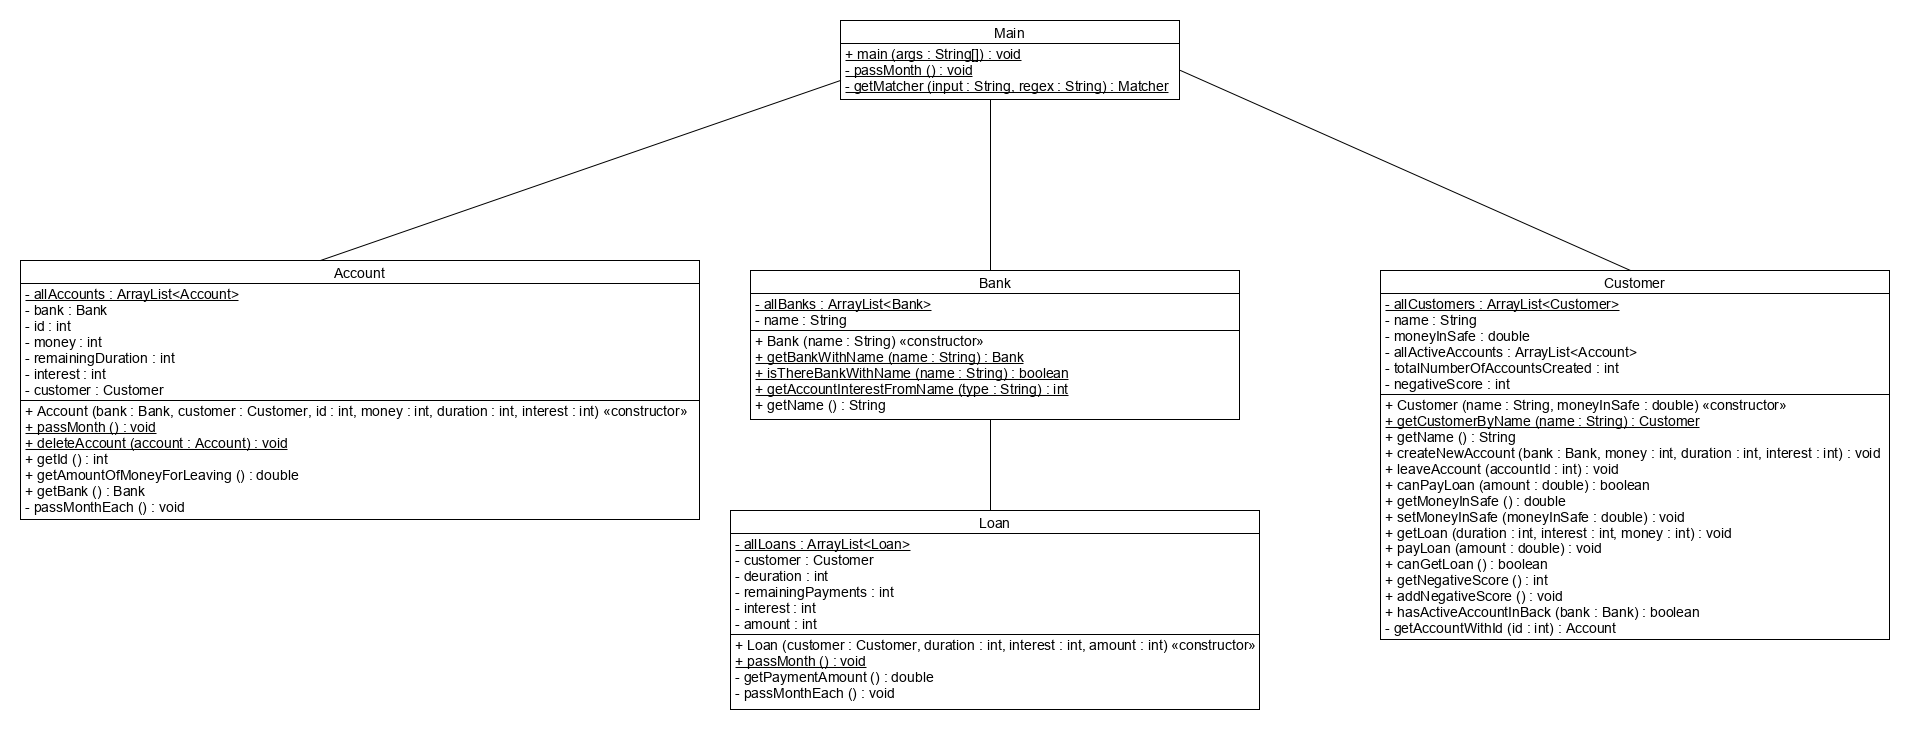
\includegraphics[width=1.8\textwidth ]{uml6.png}\\	
\end{center}
\end{changemargin}
\end{landscape}
\newpage

\section{‌شطرنج‌نامه}

ایکس و ایگرگ دو شطرنج‌باز حرفه‌ای هستند که متأسفانه در جزیره‌ای دور افتاده به همراه شما و البته یک عدد لپ تاپ (و تعدادی باطری اضافی برای لپ تاپ!) گیرافتاده اند و از آن جایی که در جزیره غذایی نیست، تصمیم دارند شما را به عنوان غذا بخورند. با این وجود از آن جایی که آن‌ها خیلی عاشق شطرنج هستند ولی هیچ مهره شطرنجی همراهشان ندارند و از طرفی هم می‌دانند که شما برنامه نویسی بلدید، به شما قول داده‌اند که اگر بتوانید کد یک بازی شطرنج را برای آن‌ها بزنید تا شطرنج‌بازی کنند، از خیر خوردن شما می‌گذرند و آن قدر بازی خواهند کرد تا خودشان از گرسنگی بمیرند! البته آن‌ها برای این که کارشان سریع‌تر راه بیفتد،‌ یکسری قوانین شطرنج را هم بی‌خیال شده‌اند و صرفاً اگر مواردی که آن‌ها از شما می‌خواهند را پیاده سازی بکنید،‌ از خیر خوردن شما خواهند گذشت.

\hrulefill
\hrulefill

همان طور که از بند بالا مشخص است، هدف شما در این سؤال پیاده سازی بازی شطرنج خواهد بود. قوانین این بازی شطرنج تا حد زیادی مشابه قوانین شطرنج واقعی است و صرفاً چند قانون آن برای سادگی حذف شده‌اند و یک مورد ویژگی متفاوت به آن اضافه شده است.

\begin{itemize}

\item در این نوع شطرنج چیزی به نام کیش و مات نداریم و صرفاً با \textbf{زدن شاه}، بازی به پایان می‌رسد. یعنی نیازی به انجام هیچ گونه چک برای کیش شدن و یا مات شدن نیست و خود بازیکنان اگر حواسشان نباشد و شاهشان در وضعیت تهدید باشد و زده شود، بازنده خواهند بود. پس از این لحاظ شما نیاز به بررسی وضعیت کیش و مات ندارید و فقط باید زده نشدن شاه بررسی شود.

\item قلعه کردن و حرکت آن پاسان در بازی وجود ندارند و نیازی به پیاده سازی آن‌ها نیست. (پیاده سازی آن‌ها نمره امتیازی هم ندارد.)


\item این موضوع که سربازها با رسیدن به آخر زمین تبدیل به وزیر و… بشوند وجود ندارد.

\item در ابتدای شروع بازی تعداد مشخصی حرکت به عنوان لیمیت تعیین خواهد شد. در صورتی که این محدودیت به اتمام برسد (یعنی دقیقاً به همان اندازه در مجموع دو نفر حرکت انجام داده باشند) و هیچ کسی بازی را برنده نشده باشد بازی مساوی اعلام می‌شود. مساوی به شکل رایج شطرنج (پات) که قوانین مختلفی نظیر تعداد و نوع مهره‌ها و حرکات ممکن و… باید در آن چک شود، در این جا وجود ندارد.

\item امکان unselect کردن مهره انتخابی برای حرکت وجود دارد و قانونی که در بین شطرنج‌بازان معروف به “دست به مهره، حرکت” است وجود ندارد.

\item قابلیت undo کردن حرکات وجود دارد (در این مورد توضیح بیش‌تری خواهیم داد).

\end{itemize}


\textbf{قوانین کلی شطرنجی که باید پیاده سازی کنید:}

شروع حرکت با مهره سفید است.

در صورت زده شدن شاه در این شطرنجی که قرار است پیاده سازی کنید، بازی به پایان رسیده و فردی که شاه را از دست داده بازی را می‌بازد. مهم‌ترین تفاوت این شطرنج با شطرنج واقعی هم همین مورد و نبودن وضعیت کیش است.

سربازها در ابتدا می‌توانند یک یا دو خانه به جلو بروند و پس از آن تنها یک خانه به جلو می‌روند. نحوه زدن مهره‌های حریف توسط سرباز به صورت ضربدری است. در حین حرکت در جلوی سرباز نباید هیچ مهره‌ای باشد.

فیل به صورت مورب حرکت می‌کند و مهره‌های دیگر را هم به همین صورت می‌زند. در حین حرکت در مسیر حرکت مورب فیل نباید هیچ مهره‌ای باشد.

حرکت رخ به صورت افقی و عمودی است و مهره‌های دیگر را هم به همین صورت می‌زند. در حین حرکت در مسیر حرکت رخ نباید هیچ مهره‌ای باشد.

حرکت وزیر مانند ترکیب حرکت رخ و فیل است و هم مورب و هم عمودی و افقی حرکت می‌کند مهره‌های دیگر را هم به همین صورت می‌زند. در حین حرکت در مسیر حرکت وزیر نباید هیچ مهره‌ای باشد.

حرکت شاه در همه جهات یعنی عمودی، افقی و مورب اما تنها یک خانه است و مهره‌های دیگر را هم به همین صورت می‌زند.

حرکت اسب به صورت L شکل است. یعنی دو خانه به جلو و یک خانه به راست یا دو خانه به جلو و یک خانه به چپ یا دو خانه به راست و یک خانه بالا و… و مهره‌های دیگر را هم به همین صورت می‌زند. در حین حرکت می‌تواند از روی سایر مهره‌ها بپرد و قرار داشتن مهره‌های دیگر در سر راه اسب مشکلی برای حرکت ایجاد نمی‌کند.


البته برنامه‌ای که باید بنویسید، صرفاً خود بازی شطرنج نیست. بلکه باید مکانیزم حساب کاربری و ثبت نام و لاگین و… را مطابق مواردی که در ادامه برای شما گفته می‌شود، پیاده سازی کنید.

\hrulefill

در این برنامه، در اصل سه منو (Menu) داریم. یکی منوی ابتدای بازی یا منوی ثبت نام است. یکی منوی اصلی و یکی هم منوی خود بازی. در ادامه به توضیح دستوراتی که در هر کدام از این منوها وارد می‌شود می‌پردازیم. توجه کنید که در هنگام شروع برنامه، به طور پیش فرض، کاربر در منوی ثبت نام قرار دارد. در تمامی منوها دستور help وجود دارد که توضیح آن را در هر منو قرار داده‌ایم. ضمناً توجه کنید تمامی پیغام‌های انجام موفقیت‌آمیز دستورات یا خطاها، در یک خط مجزا چاپ می‌شوند و بعد به خط بعدی می‌رود.

همچنین توجه کنید که نماد [] در دستورات پایین در خود دستور نوشته نمی‌شوند. صرفاً برای نمایش این که در این قسمت عبارتی از سمت کاربر باید وارد شود نوشته شده‌اند.

یعنی مثلاً یک عبارت معتبر برای



\begin{tcolorbox}[boxrule=0pt]
	\begin{latin}
  	  \large{
  	  	register [username] [password]
		}
	\end{latin}
\end{tcolorbox}

به صورت:



\begin{tcolorbox}[boxrule=0pt]
	\begin{latin}
  	  \large{
  	  	register ali 1234
		}
	\end{latin}
\end{tcolorbox}

می‌تواند باشد.

\textbf{منوی ثبت نام:}

در ابتدای شروع برنامه کاربر در این منو قرار دارد.

دستورات:



\begin{tcolorbox}[boxrule=0pt]
	\begin{latin}
  	  \large{
  	  	register [username] [password]
		}
	\end{latin}
\end{tcolorbox}

همان طور که مشخص است، یک کاربر با نام کاربری و پسورد مشخص شده را ایجاد می‌کند. نام کاربری و پسورد باید فقط شامل حروف الفبای انگلیسی، اعداد و کاراکتر آندرلاین \_ باشند. خطاهای مربوط به این دستور به این ترتیب چک می‌شوند و هر خطا که رخ داده بود، پیغام همان خطا چاپ شده و سایر خطاها بررسی نمی‌شوند. اگر هیچ خطایی رخ نداد و عملیات موفقیت‌آمیز بود، پیغام



\begin{tcolorbox}[boxrule=0pt]
	\begin{latin}
  	  \large{
  	  	register successful
		}
	\end{latin}
\end{tcolorbox}

چاپ خواهد شد.

خطاها: 

اگر نام کاربری شامل کاراکترهایی به جز کاراکترهای ذکر شده بود، پیغام:



\begin{tcolorbox}[boxrule=0pt]
	\begin{latin}
  	  \large{
  	  	username format is invalid
		}
	\end{latin}
\end{tcolorbox}

اگر پسورد شامل کاراکترهایی به جز کاراکترهای ذکر شده بود، پیغام:



\begin{tcolorbox}[boxrule=0pt]
	\begin{latin}
  	  \large{
  	  	password format is invalid
		}
	\end{latin}
\end{tcolorbox}

اگر کاربری با username گفته شده از قبل وجود داشت پیغام:



\begin{tcolorbox}[boxrule=0pt]
	\begin{latin}
  	  \large{
  	  	a user exists with this username
		}
	\end{latin}
\end{tcolorbox}

چاپ خواهد شد.

----------



\begin{tcolorbox}[boxrule=0pt]
	\begin{latin}
  	  \large{
  	  	login [username] [password]
		}
	\end{latin}
\end{tcolorbox}

برای لاگین کردن به حساب کاربری مشخص با نام کاربری و پسورد داده شده استفاده می‌شود. نام کاربری و پسورد باید فقط شامل حروف الفبای انگلیسی، اعداد و کاراکتر آندرلاین \_ باشند. خطاهای مربوط به این دستور به این ترتیب چک می‌شوند و هر خطا که رخ داده بود، پیغام همان خطا چاپ شده و سایر خطاها بررسی نمی‌شوند. اگر هیچ خطایی رخ نداد و عملیات موفقیت‌آمیز بود، پیغام


\begin{tcolorbox}[boxrule=0pt]
	\begin{latin}
  	  \large{
  	  	login successful
		}
	\end{latin}
\end{tcolorbox}

چاپ خواهد شد و پس از آن کاربر به طور خودکار وارد منوی اصلی خواهد شد.

خطاها: 

اگر نام کاربری شامل کاراکترهایی به جز کاراکترهای ذکر شده بود، پیغام:



\begin{tcolorbox}[boxrule=0pt]
	\begin{latin}
  	  \large{
  	  	username format is invalid
		}
	\end{latin}
\end{tcolorbox}

اگر پسورد شامل کاراکترهایی به جز کاراکترهای ذکر شده بود، پیغام:



\begin{tcolorbox}[boxrule=0pt]
	\begin{latin}
  	  \large{
  	  	password format is invalid
		}
	\end{latin}
\end{tcolorbox}

اگر کاربری با username گفته شده وجود نداشت:



\begin{tcolorbox}[boxrule=0pt]
	\begin{latin}
  	  \large{
  	  	no user exists with this username
		}
	\end{latin}
\end{tcolorbox}

اگر پسورد غلط بود:


\begin{tcolorbox}[boxrule=0pt]
	\begin{latin}
  	  \large{
  	  	incorrect password
		}
	\end{latin}
\end{tcolorbox}

چاپ خواهد شد.

\hrulefill




\begin{tcolorbox}[boxrule=0pt]
	\begin{latin}
  	  \large{
  	  	remove [username] [password]
		}
	\end{latin}
\end{tcolorbox}

برای حذف کردن یک حساب کاربری مشخص با نام کاربری و پسورد داده شده استفاده می‌شود. نام کاربری و پسورد باید فقط شامل حروف الفبای انگلیسی، اعداد و کاراکتر آندرلاین \_ باشند. خطاهای مربوط به این دستور به این ترتیب چک می‌شوند و هر خطا که رخ داده بود، پیغام همان خطا چاپ شده و سایر خطاها بررسی نمی‌شوند. اگر همه موفق آمیز بودند پیغام


\begin{tcolorbox}[boxrule=0pt]
	\begin{latin}
  	  \large{
  	  	removed [username] successfully
		}
	\end{latin}
\end{tcolorbox}

چاپ خواهد شد که به جای username باید نام کاربری فرد حذف شده نشان داده شود.

خطاها: 

اگر نام کاربری شامل کاراکترهایی به جز کاراکترهای ذکر شده بود، پیغام:



\begin{tcolorbox}[boxrule=0pt]
	\begin{latin}
  	  \large{
  	  	username format is invalid
		}
	\end{latin}
\end{tcolorbox}

اگر پسورد شامل کاراکترهایی به جز کاراکترهای ذکر شده بود، پیغام:


\begin{tcolorbox}[boxrule=0pt]
	\begin{latin}
  	  \large{
  	  	password format is invalid
		}
	\end{latin}
\end{tcolorbox}

اگر کاربری با username گفته شده وجود نداشت:


\begin{tcolorbox}[boxrule=0pt]
	\begin{latin}
  	  \large{
  	  	no user exists with this username
		}
	\end{latin}
\end{tcolorbox}

اگر پسورد غلط بود:



\begin{tcolorbox}[boxrule=0pt]
	\begin{latin}
  	  \large{
  	  	incorrect password
		}
	\end{latin}
\end{tcolorbox}

چاپ خواهد شد.

\hrulefill




\begin{tcolorbox}[boxrule=0pt]
	\begin{latin}
  	  \large{
  	  	list\_users
		}
	\end{latin}
\end{tcolorbox}

این دستور لیست تمامی کاربرانی که وجود دارند را به ترتیب الفبایی (Lexicographical) نمایش می‌دهد.


\hrulefill



\begin{tcolorbox}[boxrule=0pt]
	\begin{latin}
  	  \large{
  	  	help
		}
	\end{latin}
\end{tcolorbox}

این فرمان انواع دستوراتی که در این بخش قابل نمایش هستند را نمایش می‌دهد. از این دستور صرفاً برای اطمینان حاصل کردن از این که در منوی درست قرار دارید. خروجی این دستور در این منو به صورت زیر است:



\begin{tcolorbox}[boxrule=0pt]
	\begin{latin}
  	  \large{
  	  	register [username] [password]
  	  	
login [username] [password]

remove [username] [password]

list\_users

help

exit
		}
	\end{latin}
\end{tcolorbox}

\hrulefill




\begin{tcolorbox}[boxrule=0pt]
	\begin{latin}
  	  \large{
  	  	exit
		}
	\end{latin}
\end{tcolorbox}

بیانگر اتمام اجرای برنامه است و بعد از چاپ پیام



\begin{tcolorbox}[boxrule=0pt]
	\begin{latin}
  	  \large{
  	  	program ended
		}
	\end{latin}
\end{tcolorbox}

اجرای برنامه پایان می‌پذیرد.

\hrulefill

\hrulefill

\textbf{منوی اصلی:}

همان طور که گفته شد، در صورت موفقیت‌آمیز بودن login وارد این منو خواهید شد.

دستورات:

\begin{tcolorbox}[boxrule=0pt]
	\begin{latin}
  	  \large{
  	  	new\_game [username] [limit]
		}
	\end{latin}
\end{tcolorbox}

``

با این دستور یک بازی جدید شروع می‌شود. در این بخش باید username یک کاربر دیگر وارد شود و بدین ترتیب بازی با آن کاربر شروع خواهد شد. کاربری که اکنون لاگین کرده و دستور را زده است در حین بازی به عنوان مهره سفید و بازیکنی که در این دستور نام او وارد شده به عنوان مهره سیاه خواهد بود. توجه کنید که در این برنامه قرار نیست چیزی نظیر لاگین شدن همزمان دو کاربر و… را هندل کنید و همه کارها در یک برنامه و توسط یک کاربر انجام می‌شود. limit هم یک عدد است و بیانگر محدودیت تعداد حرکات (نوبت‌ها در بازی) است. اگر این عدد 0 باشد به معنی نبودن هیچ محدودیتی در بازی است. جزئیات بیش‌تر مربوط به limit در بخش مربوط به بازی توضیح داده شده‌اند.

خطاهای این دستور:

اگر username از کاراکترهایی که در منوی لاگین توضیح دادیم تشکیل نشده بود، پیام:

\begin{tcolorbox}[boxrule=0pt]
	\begin{latin}
  	  \large{
  	  	username format is invalid
		}
	\end{latin}
\end{tcolorbox}



اگر limit عددی کوچک‌تر از 0 بود:

\begin{tcolorbox}[boxrule=0pt]
	\begin{latin}
  	  \large{
  	  	number should be positive to have a limit or 0 for no limit
		}
	\end{latin}
\end{tcolorbox}



اگر کاربری که دستور را زده است، نام کاربری خودش را وارد کرد:

\begin{tcolorbox}[boxrule=0pt]
	\begin{latin}
  	  \large{
  	  	you must choose another player to start a game
		}
	\end{latin}
\end{tcolorbox}



اگر کاربری با این نام کاربری وجود نداشت:

\begin{tcolorbox}[boxrule=0pt]
	\begin{latin}
  	  \large{
  	  	no user exists with this username
		}
	\end{latin}
\end{tcolorbox}



چاپ خواهد شد.

در صورت اجرای موفقیت‌آمیز دستور، پیام:

\begin{tcolorbox}[boxrule=0pt]
	\begin{latin}
  	  \large{
  	  	new game started successfully between [first] and [second] with limit [limit]
		}
	\end{latin}
\end{tcolorbox}



جاپ می‌شود که در آن first نام کاربری بازیکن سفید و second نام کاربری بازیکن سیاه و limit هم عدد محدودیت بازی است (در حالتی که 0 وارد شده بود \- به معنی عدم محدودیت\- هم عدد 0 نمایش داده خواهد شد و استثنایی وجود ندارد.)

\hrulefill


\begin{tcolorbox}[boxrule=0pt]
	\begin{latin}
  	  \large{
  	  	scoreboard
		}
	\end{latin}
\end{tcolorbox}



پیش از توضیح خروجی این دستور باید در مورد امتیاز دهی در بازی صحبت بکنیم. هر برد معمولی (از طریق زدن شاه) 3 امتیاز و باخت به این شکل 0 امتیاز دارد. در صورتی که یکی از بازیکنان انصراف بدهد (با دستوری که در بخش مربوط به بازی توضیح می‌دهیم)، برنده بازی 2 امتیاز دریافت کرده و شخصی که انصراف داده 1 امتیاز منفی کسب می‌کند. در صورت تساوی بازی (که در اثر اتمام limit اتفاق می‌افتد) هر بازیکن 1 امتیاز می‌گیرد.

 بعد از اجرای این دستور باید کاربران با این فرمت نوشته بشوند:

\begin{tcolorbox}[boxrule=0pt]
	\begin{latin}
  	  \large{
  	  	[username] [score] [wins] [draws] [losses]
		}
	\end{latin}
\end{tcolorbox}



منظور از wins و draws و losses تعداد بردها، تساوی‌ها و باخت هاست.

ترتیب مرتب سازی کاربران هم به ترتیب از بالاترین اولویت به کمترین به این صورت است: بیش‌ترین امتیاز \- در صورت برابری امتیاز بیش‌ترین تعداد برد \- در صورت برابری تعداد برد بیش‌ترین تعداد تساوی \- در صورت برابری تساوی کمترین باخت و در صورت برابری تمامی موارد، براساس حروف الفبا (lexicographical) به طور صعودی (یعنی a زودتر از z می‌آید و…)


\hrulefill





\begin{tcolorbox}[boxrule=0pt]
	\begin{latin}
  	  \large{
  	  	list\_users
		}
	\end{latin}
\end{tcolorbox}

کاملاً مشابه همین دستور که در منوی قبلی توضیح داده شد، عمل می‌کند.

\hrulefill


\begin{tcolorbox}[boxrule=0pt]
	\begin{latin}
  	  \large{
  	  	help
		}
	\end{latin}
\end{tcolorbox}

مشابه همان چیزی است که در بخش قبل توضیح دادیم. خروجی آن عیناً به این شکل است:



\begin{tcolorbox}[boxrule=0pt]
	\begin{latin}
  	  \large{

  	  	new\_game [username] [limit]

scoreboard

list\_users

help

logout
		}
	\end{latin}
\end{tcolorbox}


\hrulefill




\begin{tcolorbox}[boxrule=0pt]
	\begin{latin}
  	  \large{
  	  	logout
		}
	\end{latin}
\end{tcolorbox}

با این دستور کاربر از حساب کاربری خود خارج می‌شود. پس از اجرای این دستور پیام


\begin{tcolorbox}[boxrule=0pt]
	\begin{latin}
  	  \large{
  	  	logout successful
		}
	\end{latin}
\end{tcolorbox}

چاپ شده و کاربر وارد منوی ثبت نام که پیش‌تر توضیح دادیم، می‌شود.

\hrulefill

\hrulefill

\textbf{منوی بازی:}

در این بخش علاوه بر این که به دستورات اشاره می‌کنیم، به موارد خاصی که باید در منطق به درستی پیاده سازی شوند هم اشاره می‌شود.

به عنوان اولین نکته به تصویر زیر که از صفحه شطرنج است توجه کنید:

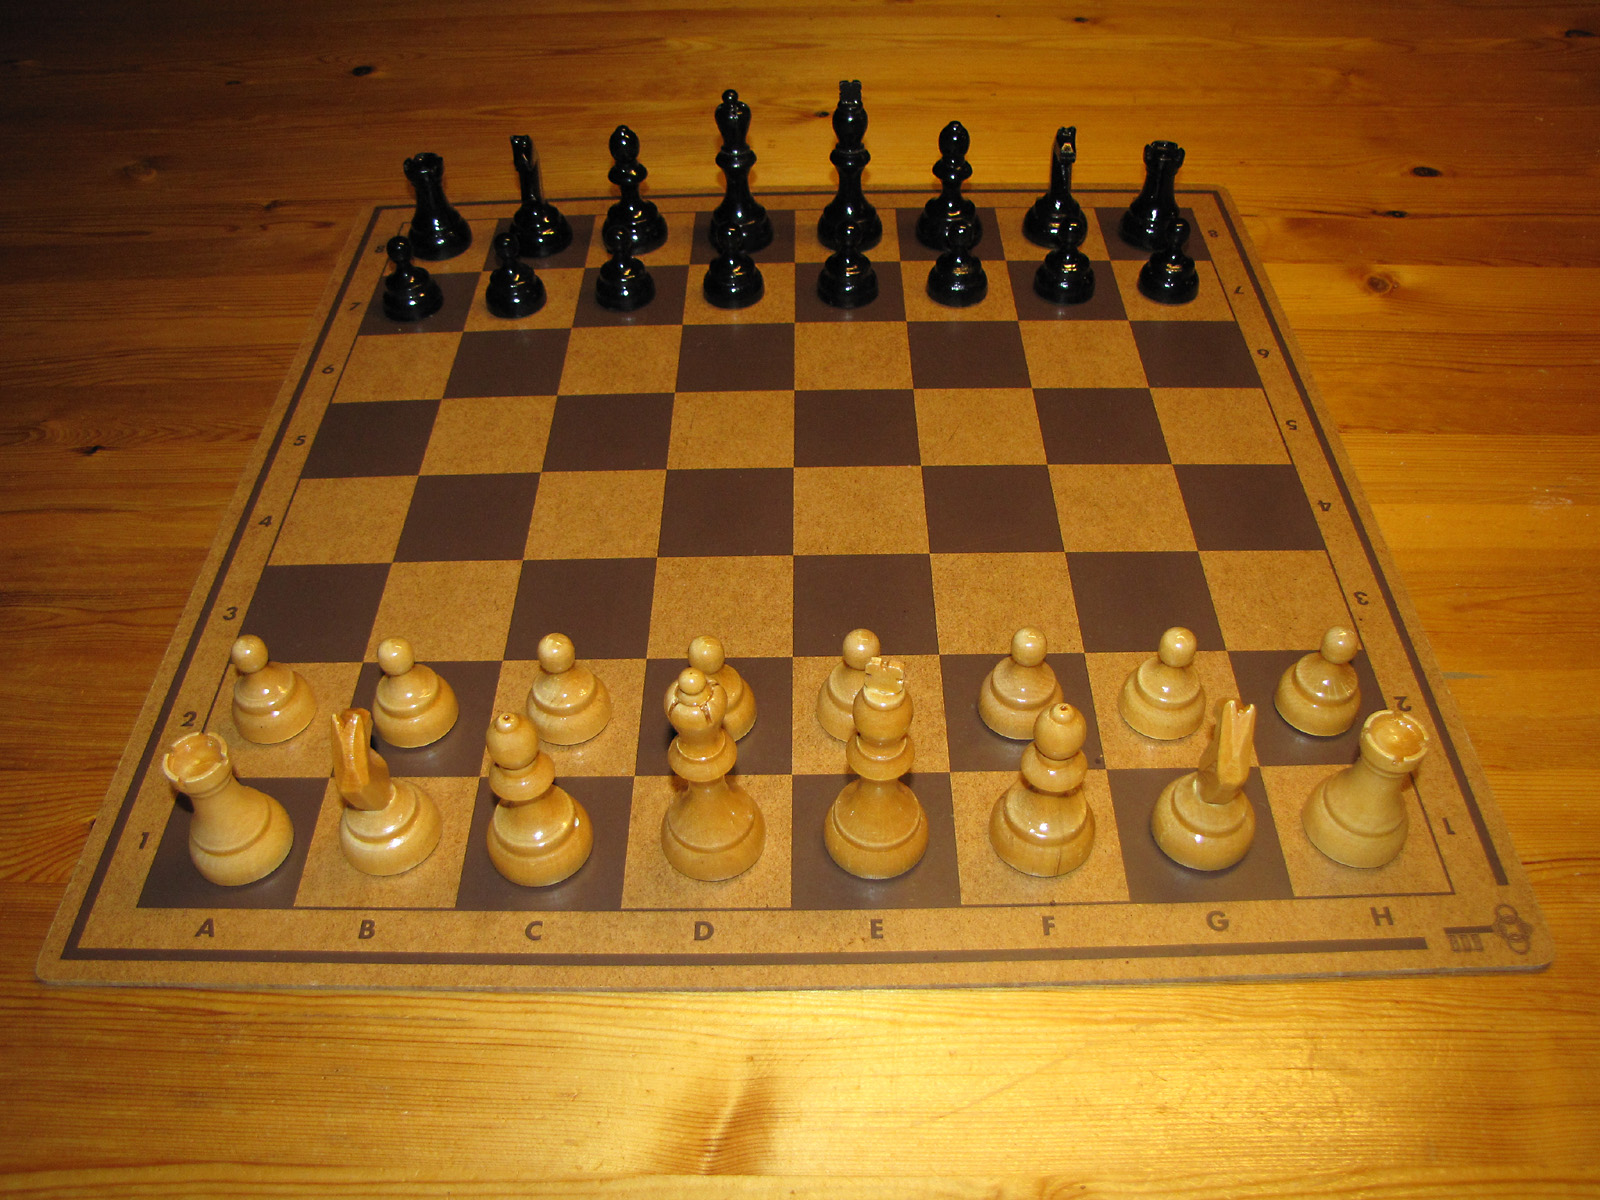
\includegraphics[width=0.8\textwidth]{chess.jpg}

 فایل تصویر به طور جداگانه باکیفیت بالاتر قرار گرفته است.

نحوه قرار گیری مهره‌ها در صفحه بازی به همین شکل خواهد بود.

در این جا اولین دستور مطرح می‌شود:


\begin{tcolorbox}[boxrule=0pt]
	\begin{latin}
  	  \large{
  	  	select [x],[y]
		}
	\end{latin}
\end{tcolorbox}

 با این دستور یک مهره را انتخاب می‌کنیم. توجه کنید که برای اشاره به یک خانه در این جا به جای حروف A تا H هم از اعداد استفاده خواهیم کرد. یعنی مثلاً در ابتدای بازی، وزیر سفید به صورت
\begin{latin}
  select 1,4
  \end{latin}
   و شاه سیاه با
   \begin{latin}
    select 8,5
    \end{latin}
     انتخاب می‌شود.

 خطاهای این دستور:

 اگر مختصات به طور کلی از محدوده خارج بود (یعنی هر مؤلفه در بازه 1 تا 8 قرار نمی‌گرفتند):



\begin{tcolorbox}[boxrule=0pt]
	\begin{latin}
  	  \large{
  	  	wrong coordination
		}
	\end{latin}
\end{tcolorbox}

اگر مهره قرار گرفته در خانه مشخص شده مربوط به حریف بود:



\begin{tcolorbox}[boxrule=0pt]
	\begin{latin}
  	  \large{
  	  	you can only select one of your pieces
		}
	\end{latin}
\end{tcolorbox}

اگر هیچ مهره‌ای در خانه نبود:



\begin{tcolorbox}[boxrule=0pt]
	\begin{latin}
  	  \large{
  	  	no piece on this spot
		}
	\end{latin}
\end{tcolorbox}

چاپ می‌شوند.

اگر هم مهره خودی در آن موقعیت بود، پیغام:


\begin{tcolorbox}[boxrule=0pt]
	\begin{latin}
  	  \large{
  	  	selected
		}
	\end{latin}
\end{tcolorbox}

چاپ می‌شود. توجه کنید که اگر یک مهره از قبل انتخاب شده باشد و بخواهیم مهره جدیدی را انتخاب کنیم، صرفاً با نوشتن دوباره دستور برای مهره جدید، مهره جدید انتخاب خواهد شد و دوباره همان خروجی


\begin{tcolorbox}[boxrule=0pt]
	\begin{latin}
  	  \large{
  	  	selected
		}
	\end{latin}
\end{tcolorbox}

را خواهیم داشت. حتی با انتخاب دوباره مهره انتخاب شده هم با همین نتیجه رو به رو خواهیم بود.

\hrulefill




\begin{tcolorbox}[boxrule=0pt]
	\begin{latin}
  	  \large{
  	  	deselect
		}
	\end{latin}
\end{tcolorbox}

این دستور باعث می‌شود مهره‌ای که در وضعیت انتخاب شده بوده، از وضعیت انتخاب شده خارج شود.

تنها خطای این دستور مربوط به وقتی است که هیچ مهره‌ای انتخاب نشده باشد و در آن صورت عبارت:


\begin{tcolorbox}[boxrule=0pt]
	\begin{latin}
  	  \large{
  	  	no piece is selected
		}
	\end{latin}
\end{tcolorbox}

چاپ می‌شود.

در صورتی هم که به درستی مهره از حالت انتخاب خارج شود، پیغام



\begin{tcolorbox}[boxrule=0pt]
	\begin{latin}
  	  \large{
  	  	deselected
		}
	\end{latin}
\end{tcolorbox}

چاپ خواهد شد.

\hrulefill



\begin{tcolorbox}[boxrule=0pt]
	\begin{latin}
  	  \large{
  	  	move [x],[y]
		}
	\end{latin}
\end{tcolorbox}

این حرکت همان طور که واضح است، باعث حرکت مهره به نقطه مشخص شده می‌شود.

خطاهای این دستور:

اگر قبل از این حرکتی در این نوبت انجام شده بود:


\begin{tcolorbox}[boxrule=0pt]
	\begin{latin}
  	  \large{
  	  	already moved
		}
	\end{latin}
\end{tcolorbox}

 اگر مختصات به طور کلی از محدوده خارج بود (یعنی هر مؤلفه در بازه 1 تا 8 قرار نمی‌گرفتند):



\begin{tcolorbox}[boxrule=0pt]
	\begin{latin}
  	  \large{
  	  	wrong coordination
		}
	\end{latin}
\end{tcolorbox}

اگر هیچ مهره‌ای انتخاب نشده بود:



\begin{tcolorbox}[boxrule=0pt]
	\begin{latin}
  	  \large{
  	  	do not have any selected piece
		}
	\end{latin}
\end{tcolorbox}

اگر خانه مورد نظر توسط مهره‌های خودی از قبل پر بود یا مانعی در مسیر برای حرکت به آن نقطه وجود داشت (مطابق قوانین شطرنج که در ابتدای داک توضیح داده شده‌اند):



\begin{tcolorbox}[boxrule=0pt]
	\begin{latin}
  	  \large{
  	  	cannot move to the spot
		}
	\end{latin}
\end{tcolorbox}

چاپ خواهد شد.

در صورت اجرای موفقیت‌آمیز، اگر حرکت به درستی انجام شد و در خانه مد نظر مهره حریف قرار داشت و زده شد عبارت:


\begin{tcolorbox}[boxrule=0pt]
	\begin{latin}
  	  \large{
  	  	rival piece destroyed
		}
	\end{latin}
\end{tcolorbox}

و اگر صرفاً حرکت انجام شد و مهره‌ای زده نشد عبارت:


\begin{tcolorbox}[boxrule=0pt]
	\begin{latin}
  	  \large{
  	  	moved
		}
	\end{latin}
\end{tcolorbox}

چاپ خواهد شد.

\hrulefill



\begin{tcolorbox}[boxrule=0pt]
	\begin{latin}
  	  \large{
  	  	next\_turn
		}
	\end{latin}
\end{tcolorbox}

نوبت را به حریف منتقل می‌کند و در صورت اجرای موفقت آمیز پیغام:



\begin{tcolorbox}[boxrule=0pt]
	\begin{latin}
  	  \large{
  	  	turn completed
		}
	\end{latin}
\end{tcolorbox}

چاپ می‌شود. توجه کنید که طبق قوانین شطرنج هر نفر باید در نوبت خود حتماً یک حرکت انجام بدهد. بنابراین اگر هیچ حرکتی انجام نشده بود، پیغام خطای:



\begin{tcolorbox}[boxrule=0pt]
	\begin{latin}
  	  \large{
  	  	you must move then proceed to next turn
		}
	\end{latin}
\end{tcolorbox}

نوشته شود.

\hrulefill



\begin{tcolorbox}[boxrule=0pt]
	\begin{latin}
  	  \large{
  	  	show\_turn
		}
	\end{latin}
\end{tcolorbox}

این دستور برای مشخص شدن این است که نوبت کدام بازیکن است. خروجی آن به فرم زیر است:



\begin{tcolorbox}[boxrule=0pt]
	\begin{latin}
  	  \large{
  	  	it is player [username] turn with color [white\\black]
		}
	\end{latin}
\end{tcolorbox}


\hrulefill



\begin{tcolorbox}[boxrule=0pt]
	\begin{latin}
  	  \large{
  	  	undo
		}
	\end{latin}
\end{tcolorbox}

یکی از ویژگی‌های منحصر به فرد شطرنجی که باید پیاده سازی کنید، قابلیت undo است. هر بازیکن در کل طول یک بازی می‌تواند دو بار از این قابلیت و در هر نوبت حداکثر یک بار استفاده کند. این قابلیت بدین صورت است که اگر بازیکنی حرکتی انجام داده باشد، در صورتی که بخواهد و طبق شرایط بالا تعداد دفعات استفاده‌اش تمام نشده باشد، حرکت خود را برگرداند. توجه کنید که چون تغییر نوبت با next\_turn انجام می‌شود، همچنان بعد از حرکت نوبت با بازیکن فعلی است تا زمانی که دستور next\_turn زده شود.

خطاهای این دستور:

اگر پیش‌تر به اندازه تعداد کل undo های مجاز (یعنی 2) بار از این قابلیت استفاده شده باشد.


\begin{tcolorbox}[boxrule=0pt]
	\begin{latin}
  	  \large{
  	  	you cannot undo anymore
		}
	\end{latin}
\end{tcolorbox}

اگر بازیکن در این نوبت حرکتی انجام نداده باشد که بخواهد undo کند:


\begin{tcolorbox}[boxrule=0pt]
	\begin{latin}
  	  \large{
  	  	you must move before undo
		}
	\end{latin}
\end{tcolorbox}

اگر در همین نوبت از undo استفاده کرده باشد:



\begin{tcolorbox}[boxrule=0pt]
	\begin{latin}
  	  \large{
  	  	you have used your undo for this turn
		}
	\end{latin}
\end{tcolorbox}

چاپ خواهند شد.

در صورت اجرای درست دستور نیز باید عبارت:


\begin{tcolorbox}[boxrule=0pt]
	\begin{latin}
  	  \large{
  	  	undo completed
		}
	\end{latin}
\end{tcolorbox}

چاپ بشود.

توجه کنید که بعد از اجرای undo، مهره‌ای که از قبل select شده همچنان در همین حالت باقی می‌ماند.


\hrulefill


\begin{tcolorbox}[boxrule=0pt]
	\begin{latin}
  	  \large{
  	  	undo\_number
		}
	\end{latin}
\end{tcolorbox}

تعداد دفعات باقی مانده undo یک بازیکن را نشان می‌دهد. در ابتدای بازی این عدد دو است و با انجام حرکت undo کاهش می‌یابد تا در نهایت بعد از دو بار انجام این حرکت، به صفر می‌رسد. فرم پیام خروجی به صورت:


\begin{tcolorbox}[boxrule=0pt]
	\begin{latin}
  	  \large{
  	  	you have [n] undo moves
		}
	\end{latin}
\end{tcolorbox}

خواهد بود که n تعداد undo های باقی مانده است.

\hrulefill

برای دستورات بعدی باید توضیحی در مورد نحوه نمایش نام هر مهره در بازی بدهیم.

نام مهره‌ها در بازی به این صورت است که ابتدا حرف اختصاری نوع مهره با حروف بزرگ و سپس رنگ مهره با حروف کوچک آورده می‌شود.

حرف اختصاری مهره‌ها بدین شرح است: سرباز P - رخ R - اسب N - فیل B - وزیر Q و شاه K. به عنوان مثال شاه سفید با علامت Kw شناخته می‌شود.

حال به توضیح خود دستور می‌پردازیم:


\begin{tcolorbox}[boxrule=0pt]
	\begin{latin}
  	  \large{
  	  	show\_moves
		}
	\end{latin}
\end{tcolorbox}

این دستور کل حرکاتی را که بازیکن فعلی انجام داده است، به ترتیب با این فرمت نمایش می‌دهد: (منظور از بازیکن فعلی، بازیکنی است که در هنگام زده شدن دستور نوبت اوست)

اگر در طول فرآیند حرکت مهره‌ای زده نشده باشد:



\begin{tcolorbox}[boxrule=0pt]
	\begin{latin}
  	  \large{
  	  	[Name of Piece that moved] [x],[y] to [x],[y]
		}
	\end{latin}
\end{tcolorbox}

اگر مهره‌ای زده شده باشد:




\begin{tcolorbox}[boxrule=0pt]
	\begin{latin}
  	  \large{
  	  	[Name of Piece that moved] [x],[y] to [x],[y] destroyed [Name of piece destroyed]
		}
	\end{latin}
\end{tcolorbox}


به عنوان مثال اگر سرباز سفید با حرکت از ردیف 4 و ستون 1 به ردیف 5 و ستون 2 رفته باشد و در این فرآیند سرباز سیاه را از بین برده باشد، حرکت به صورت



\begin{tcolorbox}[boxrule=0pt]
	\begin{latin}
  	  \large{
  	  	Pw 4,1 to 5,2 destroyed Pb
		}
	\end{latin}
\end{tcolorbox}

نمایش داده خواهد شد.

\hrulefill


\begin{tcolorbox}[boxrule=0pt]
	\begin{latin}
  	  \large{
  	  	show\_moves -all
		}
	\end{latin}
\end{tcolorbox}

این دستور مشابه دستور قبلی است با این تفاوت که حرکات تمامی بازیکنان را به ترتیب از ابتدای شروع بازی نمایش می‌دهد.

\hrulefill



\begin{tcolorbox}[boxrule=0pt]
	\begin{latin}
  	  \large{
  	  	show\_killed
		}
	\end{latin}
\end{tcolorbox}


این دستور مهره‌های زده شده بازیکن فعلی را نشان می‌دهد. (یعنی مهره‌هایی از او که حریف آن‌ها را زده است).

فرمت نمایش آن‌ها به این صورت است:


\begin{tcolorbox}[boxrule=0pt]
	\begin{latin}
  	  \large{
  	  	[Name of Piece] killed in spot [x],[y]
		}
	\end{latin}
\end{tcolorbox}


ترتیب نمایش مهره‌ها، به ترتیب زمان زده شدن است. (مهره‌ای که زودتر زده شده، زودتر نمایش داده می‌شود)

\hrulefill



\begin{tcolorbox}[boxrule=0pt]
	\begin{latin}
  	  \large{
  	  	show\_killed -all
		}
	\end{latin}
\end{tcolorbox}

مشابه دستور بالاست ولی همه مهره‌های زده شده در بازی را به ترتیب زده شدن نمایش می‌دهد.

\hrulefill



\begin{tcolorbox}[boxrule=0pt]
	\begin{latin}
  	  \large{
  	  	show\_board
		}
	\end{latin}
\end{tcolorbox}

این دستور صفحه شطرنج را به همراه مهره‌های حاضر در آن نمایش می‌دهد. برای مثال در ابتدای بازی فرمت نمایش صفحه به صورت زیر است و به طور کلی باید به همین شکل نمایش بدهید.




\begin{tcolorbox}[boxrule=0pt]
	\begin{latin}
  	  \large{
  	  	Rb|Nb|Bb|Qb|Kb|Bb|Nb|Rb|
  	  	
Pb|Pb|Pb|Pb|Pb|Pb|Pb|Pb|

~~  | ~~ | ~~ | ~~ | ~~ | ~~ | ~~ | ~~ |
  
~~  | ~~ | ~~ | ~~ | ~~ | ~~ | ~~ | ~~ |
  
~~  | ~~ | ~~ | ~~ | ~~ | ~~ | ~~ | ~~ |
  
~~  | ~~ | ~~ | ~~ | ~~ | ~~ | ~~ | ~~ |
  
Pw|Pw|Pw|Pw|Pw|Pw|Pw|Pw|

Rw|Nw|Bw|Qw|Kw|Bw|Nw|Rw|

		}
	\end{latin}
\end{tcolorbox}



توجه کنید که خانه‌های خالی با دو اسپیس نمایش داده می‌شوند. در صورتی که می‌خواهید عیناً ساختار بالا را کپی کنید، به صفحه کوئرا مراجعه کنید.


یعنی زاویه دید، مشابه عکسی است که بالاتر از بازی شطرنج نمایش دادیم و سفید در پایین تصویر و سیاه در بالای تصویر خواهد بود.

\hrulefill
\newpage

\begin{tcolorbox}[boxrule=0pt]
	\begin{latin}
  	  \large{
  	  	help
		}
	\end{latin}
\end{tcolorbox}

مشابه دستور help در سایر بخش‌هاست. در این جا باید عیناً این خروجی نمایش داده شود:



\begin{tcolorbox}[boxrule=0pt]
	\begin{latin}
  	  \large{
  	  	select [x],[y]
  	  	
deselect

move [x],[y]

next\_turn

show\_turn

undo

undo\_number

show\_moves [-all]

show\_killed [-all]

show\_board

help

forfeit
		}
	\end{latin}
\end{tcolorbox}

\hrulefill



\begin{tcolorbox}[boxrule=0pt]
	\begin{latin}
  	  \large{
  	  	forfeit
		}
	\end{latin}
\end{tcolorbox}

این دستور مربوط به انصراف از بازی می‌شود و بازیکنی که این دستور را وارد کند، بازنده بازی خواهد بود و نفر دیگر برنده بازی خواهد بود. همان طور که بالاتر گفتیم، با این اتفاق، حریف که برنده بازی شده، 2 امتیاز می‌گیرد و کسی که انصراف داده منفی 1 امتیاز دریافت می‌کند (یعنی 1 امتیاز از او کم می‌شود).

بعد از اجرای این دستور باید این دو پیام در دو خط پشت سرهم نمایش داده شوند:



\begin{tcolorbox}[boxrule=0pt]
	\begin{latin}
  	  \large{
  	  	you have forfeited
		}
	\end{latin}
\end{tcolorbox}




\begin{tcolorbox}[boxrule=0pt]
	\begin{latin}
  	  \large{
  	  	player [username] with color [black\/white] won
		}
	\end{latin}
\end{tcolorbox}


و به جای username و black/white هم نام کاربری و رنگ بازیکن برنده قرار می‌گیرد. پس از آن هم کاربر به منوی اصلی بازگردانده می‌شود.

بدین ترتیب توصیف دستورات به پایان رسید. صرفاً باید مواردی را در مورد پایان بازی ذکر کنیم.

\hrulefill

در صورتی که شاه حریف زده شود، بازی به نفع شخصی که شاه حریف را زده است، تمام می‌شود. این موضوع که شاه حریف زده شده در دستور next\_turn بررسی می‌شود.

در صورت اتمام بازی با برد یکی از طرفین پیامی به صورت:



\begin{tcolorbox}[boxrule=0pt]
	\begin{latin}
  	  \large{
  	  	player [username] with color [black\/white] won
		}
	\end{latin}
\end{tcolorbox}

چاپ می‌شود.

در مورد شرایط تساوی، همان طور که گفته شد، تنها باید وضعیت limit تعداد حرکات را بررسی بکنید. با گذشت هر نوبت به نوعی یک واحد به limit مد نظر نزدیک‌تر می‌شویم. یعنی به نوعی اگر limit عدد 20 باشد، هر یک از طرفین می‌تواند 10 نوبت بازی کند. در این مثال، اگر بعد از گذشت 20 نوبت در کل، هیچ یک از طرفین برنده بازی نشد، بازی با تساوی به اتمام می‌رسد. توجه کنید که اگر limit برابر 0 باشد، یعنی هیچ محدودیتی نیست و بازی کلاً با تساوی به اتمام نخواهد رسید. در صورت تساوی عبارت زیر چاپ می‌شود:



\begin{tcolorbox}[boxrule=0pt]
	\begin{latin}
  	  \large{
  	  	draw
		}
	\end{latin}
\end{tcolorbox}

و کاربر به منو اصلی باز گردانده می‌شود.

همان طور که پیش‌تر هم گفتیم، در اثر تساوی به هر کدام از بازیکنان 1 امتیاز داده می‌شود.

با توجه به توضیحات بالا نیازی به چک کردن شرایط واقعی تساوی در شطرنج ندارید.

در نهایت توجه کنید که اگر در هر کدام از منوها، دستوری زده شود که با دستورات آن منو تطابق نداشته باشد، باید پیام 



\begin{tcolorbox}[boxrule=0pt]
	\begin{latin}
  	  \large{
  	  	invalid command
		}
	\end{latin}
\end{tcolorbox}

در یک خط چاپ شود و به خط بعدی برویم.

در مورد خطاهای دستورات، توجه کنید که ترتیب چک شدن آن‌ها به ترتیبی است که در این داک نوشته شده‌اند و در صورت رخ دادن اولین خطا و چاپ پیام خطا، سایر خطاها بررسی نمی‌شوند.


\newpage
\section{نصّاب پنجره}
وینیسیوس جونیور که در پی ویروس کرونا خانه نشین شده است تصمیم گرفته تا سیستم عامل لپ تاپ خود را تغییر دهد؛ اما چون تجربه‌ای در این کار ندارد از شما کمک خواسته است. در این سؤال شما بایستی دستوراتی که او به شما می‌دهد را پیاده کنید.
در این سؤال ابتدا با نصب سیستم عامل و ساخت درایو ها شروع کرده سپس به سراغ ساخت فایل و فولدر و کارهای مربوط به آن‌ها خواهیم رفت؛ اما ابتدا یکسری نکات کلی در مورد این سؤال:

در مورد فایل:

در این سؤال با 3 مدل فایل سروکار داریم عکس (فرمت $img$)، ویدئو (فرمت $mp4$) و متن (فرمت $txt$) هستند.

یک سری ویژگی‌ها در تمام این نوع فایل‌ها وجود دارند مانند آدرس و اسم و ….	. که در ادامه با دستورات مربوط به آن‌ها آشنا می‌شوید. اما بعضی ویژگی‌ها هستند که بنا بر نوع فایل متفاوت‌اند. این ویژگی‌ها به ترتیب برای هر فایل به شکل زیر هستند:

ویدیو:

\begin{latin}
 Quality(240p, 360p,720p,1080p,2160p)
 
Video Length
\end{latin}
(که به فرمت hh:mm:ss داده می‌شه)

متن:
\begin{latin}
Text
\end{latin}
(نگران نباشین قرار نیست با فایل متنی واقعی کار کنین صرفاً کافیه یه رشته در نظر بگیرین براش)


عکس:
\begin{latin}
Resolution
\end{latin}
(به صورت دو عدد با علامت * در بینشون مثل $1536*2048$)



\begin{latin}
Extension(jpg, png)
\end{latin}


در مورد فولدر:

هر فولدر از تعدادی فایل و فولدر دیگر تشکیل شده است.

نکته مهم: توجه کنید که در هر بخش اگر دستور ورودی طبق فرمت داده شده نبود کافی است دستور خطای گفته شده را چاپ کنید و برنامه در همان بخش باقی می‌ماند.

نکته مهم 2: دقت کنید که ارورهایی که برای هر دستور در ادامه گفته شده را به همین ترتیب داک، چک کنید


نکته مهم 3: نام فایل‌ها و فولدرها case sensitive نیست و در واقع دو فولدر a و A نمی‌توانند در یک مکان باشند (برای دو فایل نیز به همین شکل)(در ادامه درباره این ارور توضیح داده شده)


نکته مهم 4: با توجه به نکته 3 در نظر داشته باشید که هر جایی که نیاز است تا اسم یک فایل و فولدر (و نه درایو) را بررسی کنید مهم نیست که حروف آن اسم بزرگ باشد یا کوچک، به عنوان مثال اگر در فولدری هستید که فایلی به نام
$AdvaNCe$
 دارید اگر دستور
 $delete~ file ~aDVanCE$
 وارد شود، دستور معتبری است (در ادامه توضیح داده شده است)


نکته مهم 5: از space های اضافی در ابتدا و انتهای دستورات صرف نظر کنید یعنی دستور $~~~~~~end~~~~~~$
نیز صحیح تلقی می‌شود.(این دستور را در انتهای توضیحات سؤال می‌توانید ببینید)

خب بریم سراغ دستورات (به کوچکی و بزرگی حروف دستورات و ارور های که باید چاپ کنید، دقت کنید):

در ابتدا دستوری برای نصب سیستم عامل به فرمت زیر وارد می‌شود (ورژن سیستم عامل می‌تواند شامل کاراکترهای غیر عدد نیز باشد ولی شامل space نیست) این دستور تضمین می‌شود که فقط یک بار وارد شود.(البته الزاماً دستور اول برنامه، این دستور نیست و باید معتبر بودن آن را چک کنید)

\begin{tcolorbox}[boxrule=0pt]
	\begin{latin}
  	  \large{
  	  	install OS \#name \#version
		}
	\end{latin}
\end{tcolorbox}

سپس دو عدد در یک خط با یک فاصله وارد می‌شوند که به ترتیب (از چپ) نشان دهنده حجم هارد و تعداد درایوهای سیستم هستند (حجم هارد را در مقیاس MB در نظر بگیرید و دقیقاً برابر با عدد داده شده (از توان 2 نبودن آن چشم پوشی کنید)) این دستور تضمین می‌شود که فقط یک بار وارد شود.(البته الزاماً دستوری که بلافاصله بعد دستور بالا وارد می‌شود، این دستور نیست و باید معتبر بودن آن را چک کنید)

\begin{tcolorbox}[boxrule=0pt]
	\begin{latin}
  	  \large{
  	  	\#hardSize \#drivesNum
		}
	\end{latin}
\end{tcolorbox}


سپس در \#drivesNum خط در هر خط یک حرف بزرگ انگلیسی داده می‌شود ($A-Z$) که نام هر درایو را نشان می‌دهد سپس با یک فاصله حجم مورد نظر برای آن درایو وارد می‌شود.(فقط عدد و بدون MB است و حتی می‌تواند صفر باشد) توجه کنید که نباید نام درایو ها تکراری باشند.

توجه: اولین درایوی که وارد می‌شود و معتبر باشد، به عنوان درایو سیستم در نظر گرفته می‌شود که به این معنی است که در ابتدای برنامه پس از ورود به محیط سیستم عامل، در داخل آن درایو قرار داریم

\begin{tcolorbox}[boxrule=0pt]
	\begin{latin}
  	  \large{
  	  	\#driveName \#driveSize
		}
	\end{latin}
\end{tcolorbox}


اگر نام وارد شده تکراری بود یا بیش از یک حرف داشت یا شامل کاراکترهای دیگری غیر از حروف بزرگ بود باید ارور زیر چاپ شود:

\begin{tcolorbox}[boxrule=0pt]
	\begin{latin}
  	  \large{
  	  	invalid name
		}
	\end{latin}
\end{tcolorbox}

اگر حجم درایو داده شده + مجموع  حجم درایو های ثبت شده قبلی از حجم هارد بیشتر بود ارور زیر چاپ شود:



\begin{tcolorbox}[boxrule=0pt]
	\begin{latin}
  	  \large{
  	  	insufficient hard size
		}
	\end{latin}
\end{tcolorbox}
تضمین می‌شود که مجموع اندازه درایو ها از اندازه هارد کمتر نخواهد بود (اگر بیشتر باشد ارور بالا را باید چاپ کنید اگر مساوی بود برنامه ادامه می‌یابد)

حال که سیستم عامل با موفقیت نصب شد وقتشه که شروع کنیم به ساخت فایل و فولدر و کار کردن با اون‌ها

\begin{tcolorbox}[boxrule=0pt]
	\begin{latin}
  	  \large{
  	  	open \#folderName
		}
	\end{latin}
\end{tcolorbox}




با این دستور وارد فولدر با اسم داده شده می‌شوید (در صورت معتبر بودن دستور، باز کردن فولدر به این معنی است که مکان فعلی تغییر می‌کند و وارد آن فولدر می‌شوید)


توجه: این دستور برای فایل‌ها وجود ندارد و حتی در صورتی که فایل با اسم داده شده نیز وجود داشته باشد اجرا نمی‌شود.


اگر فولدری با نام داده شده در آن مکان وجود نداشت باید ارور زیر چاپ شود
\begin{tcolorbox}[boxrule=0pt]
	\begin{latin}
  	  \large{
  	  	invalid name
		}
	\end{latin}
\end{tcolorbox}




\begin{tcolorbox}[boxrule=0pt]
	\begin{latin}
  	  \large{
  	  	go to drive \#driveName
		}
	\end{latin}
\end{tcolorbox}
این دستور در هر کجای برنامه وارد شود بایستی وارد درایو با نام داده شده شوید به این معنی که مکان فعلی تغییر می‌کند و وارد آن درایو می‌شوید.

اگر درایوی با نام داده شده وجود نداشت باید ارور زیر چاپ شود

\begin{tcolorbox}[boxrule=0pt]
	\begin{latin}
  	  \large{
  	  	invalid name
		}
	\end{latin}
\end{tcolorbox}




\begin{tcolorbox}[boxrule=0pt]
	\begin{latin}
  	  \large{
  	  	back
		}
	\end{latin}
\end{tcolorbox}


با این دستور یک مرحله به عقب برمی‌گردید.

مثال:


اگر مکان فعلی

\begin{tcolorbox}[boxrule=0pt]
	\begin{latin}
  	  \large{
  	  	 H:\textbackslash APSpirng98\textbackslash HW3
		}
	\end{latin}
\end{tcolorbox}

 
  باشد و دستور back وارد شود، مکان به
  
  \begin{tcolorbox}[boxrule=0pt]
	\begin{latin}
  	  \large{
  	  	 H:\textbackslash APSpirng98 
		}
	\end{latin}
\end{tcolorbox}
   
   
   تغییر می‌کند
   
   
مثال 2:
اگر مکان فعلی
 H:\textbackslash
 باشد و دستور back وارد شود، مکان شما تغییر نمی‌کند و اروری نیز چاپ نمی‌شود.
 
  \begin{tcolorbox}[boxrule=0pt]
	\begin{latin}
  	  \large{
  	  	create folder \#name
		}
	\end{latin}
\end{tcolorbox}

با دستور بالا فولدری با اسم داده شده در مکان فعلی ساخته می‌شود. نام فولدر می‌تواند شامل کاراکترهای غیر حروف نیز باشد

 اگر فولدر دیگری با آن اسم در آن مکان وجود داشت ارور زیر چاپ شود:
 


  \begin{tcolorbox}[boxrule=0pt]
	\begin{latin}
  	  \large{
  	  	folder exists with this name
		}
	\end{latin}
\end{tcolorbox}

اگر دستور معتبر بود پس از ساخت فولدر عبارت زیر چاپ شود:

  \begin{tcolorbox}[boxrule=0pt]
	\begin{latin}
  	  \large{
  	  folder created
		}
	\end{latin}
\end{tcolorbox}

  \begin{tcolorbox}[boxrule=0pt]
	\begin{latin}
  	  \large{
  	 create file \#name \#format \#size
		}
	\end{latin}
\end{tcolorbox}






با دستور بالا فایلی با اسم داده شده در مکان فعلی ساخته می‌شود. سایز داده شده برحسب MB است. نام فایل می‌تواند شامل کاراکترهای غیر حروف نیز باشد.

اگر فایل دیگری با آن اسم در آن مکان وجود داشت ارور زیر چاپ شود:

  \begin{tcolorbox}[boxrule=0pt]
	\begin{latin}
  	  \large{
  	 file exists with this name
		}
	\end{latin}
\end{tcolorbox}



اگر فرمت داده شده از 3 نوع $mp4$, $img$, $txt$ نبود باید ارور زیر چاپ شود:

  \begin{tcolorbox}[boxrule=0pt]
	\begin{latin}
  	  \large{
  	 invalid format
		}
	\end{latin}
\end{tcolorbox}




اگر حجم فایل داده شده + حجم فایل‌های داخل آن درایو از حجم آن درایو بیشتر بود (فضای کافی برای ساخت فایل وجود نداشت) باید ارور زیر چاپ شود:

 \begin{tcolorbox}[boxrule=0pt]
	\begin{latin}
  	  \large{
  	 insufficient drive size
		}
	\end{latin}
\end{tcolorbox}

توجه کنید که format معتبر داده شده یکی از 3 نوع $mp4$,$img$, $txt$ است که بسته به اینکه کدام نوع باشد باید فایلی از نوع متن، عکس یا ویدیو بسازید.

سپس اگر ورودی مشکلی نداشت، به نسبت فرمت فایل، معیارها را دریافت می‌کند. به این صورت که به ترتیب آورده شده در بالا، معیارها چاپ می‌شود و مقادیر مورد نظر از ورودی دریافت می‌شود. 

مثلاً اگر ویدیو بود باید چاپ کنید:

 \begin{tcolorbox}[boxrule=0pt]
	\begin{latin}
  	  \large{
  	 Quality:
		}
	\end{latin}
\end{tcolorbox}


سپس ورودی بگیرید و سپس چاپ کنید:

 \begin{tcolorbox}[boxrule=0pt]
	\begin{latin}
  	  \large{
  	Video Length:
		}
	\end{latin}
\end{tcolorbox}


و ورودی بگیرید.(تضمین می‌شود که این ورودی‌ها معتبر باشند)

در نهایت اگر دستور معتبر بود پس از گرفتن ویژگی‌های فایل که در بالا گفته شد، و پس از ساخت فایل عبارت زیر چاپ شود:

 \begin{tcolorbox}[boxrule=0pt]
	\begin{latin}
  	  \large{
  	file created
		}
	\end{latin}
\end{tcolorbox}


\begin{tcolorbox}[boxrule=0pt]
	\begin{latin}
  	  \large{
  	delete file \#fileName
		}
	\end{latin}
\end{tcolorbox}


با این دستور فایل با اسم داده را حذف می‌کنید و حجم آن را نیز از حجم استفاده شده از فضای درایو حذف می‌کنید.

اگر فایلی با نام داده شده در آن مکان وجود نداشت باید ارور زیر چاپ شود:

\begin{tcolorbox}[boxrule=0pt]
	\begin{latin}
  	  \large{
  	invalid name
		}
	\end{latin}
\end{tcolorbox}


اگر دستور معتبر بود پس از حذف فایل عبارت زیر چاپ شود:

\begin{tcolorbox}[boxrule=0pt]
	\begin{latin}
  	  \large{
  	file deleted
		}
	\end{latin}
\end{tcolorbox}



\begin{tcolorbox}[boxrule=0pt]
	\begin{latin}
  	  \large{
  	delete folder \#folderName
		}
	\end{latin}
\end{tcolorbox}


با این دستور فولدر با اسم داده را حذف می‌کنید. دقت کنید که با حذف فولدر تمام فایل‌ها و فولدرهای داخل آن نیز حذف خواهند شد.

اگر فولدری با نام داده شده در آن مکان وجود نداشت باید ارور زیر چاپ شود:

\begin{tcolorbox}[boxrule=0pt]
	\begin{latin}
  	  \large{
  	invalid name
		}
	\end{latin}
\end{tcolorbox}



اگر دستور معتبر بود پس از حذف فولدر عبارت زیر چاپ شود:

\begin{tcolorbox}[boxrule=0pt]
	\begin{latin}
  	  \large{
  	folder deleted
		}
	\end{latin}
\end{tcolorbox}







\begin{tcolorbox}[boxrule=0pt]
	\begin{latin}
  	  \large{
  	rename file \#fileName \#newName
		}
	\end{latin}
\end{tcolorbox}


اسم فایل با اسم داده شده را تغییر می‌دهید.
اگر فایلی با نام داده شده در آن مکان وجود نداشت باید ارور زیر چاپ شود:



\begin{tcolorbox}[boxrule=0pt]
	\begin{latin}
  	  \large{
  	invalid name
		}
	\end{latin}
\end{tcolorbox}



اگر فایل دیگری به نام \#newName در آن مکان وجود داشت باید ارور زیر چاپ شود:

\begin{tcolorbox}[boxrule=0pt]
	\begin{latin}
  	  \large{
  	file exists with this name
		}
	\end{latin}
\end{tcolorbox}



اگر دستور معتبر بود پس از تغییر نام فایل عبارت زیر چاپ شود:

\begin{tcolorbox}[boxrule=0pt]
	\begin{latin}
  	  \large{
  	file renamed
		}
	\end{latin}
\end{tcolorbox}


\begin{tcolorbox}[boxrule=0pt]
	\begin{latin}
  	  \large{
  	rename folder \#folderName \#newName
		}
	\end{latin}
\end{tcolorbox}

اسم فولدر با اسم داده شده را تغییر می‌دهید.
اگر فولدر با نام داده شده در آن مکان وجود نداشت باید ارور زیر چاپ شود:

\begin{tcolorbox}[boxrule=0pt]
	\begin{latin}
  	  \large{
  	invalid name
		}
	\end{latin}
\end{tcolorbox}

اگر فولدر دیگری به نام \#newName در آن مکان وجود داشت باید ارور زیر چاپ شود:


\begin{tcolorbox}[boxrule=0pt]
	\begin{latin}
  	  \large{
  	folder exists with this name
		}
	\end{latin}
\end{tcolorbox}

اگر دستور معتبر بود پس از تغییر نام فولدر عبارت زیر چاپ شود:

\begin{tcolorbox}[boxrule=0pt]
	\begin{latin}
  	  \large{
  	folder renamed
		}
	\end{latin}
\end{tcolorbox}



\begin{tcolorbox}[boxrule=0pt]
	\begin{latin}
  	  \large{
  	status
		}
	\end{latin}
\end{tcolorbox}


این دستور اگر هنگامی که داخل درایو یا فولدری هستیم وارد شود ابتدا در یک خط آدرس مکان فعلی را چاپ کنید به عنوان مثال:

\begin{tcolorbox}[boxrule=0pt]
	\begin{latin}
  	  \large{
  	H:\textbackslash Java‍~Projects\textbackslash  APSpirng98\textbackslash HW3
		}
	\end{latin}
\end{tcolorbox}

 
سپس نام تمام فایل‌ها و فولدرهای آن مکان را به ترتیب نام و به فرمت زیر چاپ کنید (به ترتیب ابتدا فولدرها و سپس عکس‌ها، متن‌ها، ویدیوها):

هر خط شامل یک اسم، فاصله، نوع آن فایل یا فولدر، فاصله، حجم آن فایل یا فولدر
به عنوان مثال:

\begin{tcolorbox}[boxrule=0pt]
	\begin{latin}
  	  \large{
  Folders:
  
Q2 50MB

q1 15MB

Files:

x img 2MB

a txt 80MB

B mp4 400MB
		}
	\end{latin}
\end{tcolorbox}


\begin{tcolorbox}[boxrule=0pt]
	\begin{latin}
  	  \large{
  	print drives status
		}
	\end{latin}
\end{tcolorbox}

در صورت وارد شدن این دستور باید به فرمت زیر اطلاعات درایو ها را چاپ کنید:
هر خط شامل اسم درایو، فاصله، حجم کلی آن درایو، فاصله، حجم اشغال شده آن درایو
توجه: ترتیب درایو ها همان ترتیب ساخته شدن آن‌ها باید باشد.


به عنوان مثال:

\begin{tcolorbox}[boxrule=0pt]
	\begin{latin}
  	  \large{
  	C 75000MB 48000MB
  	
H 100000MB 500MB

		}
	\end{latin}
\end{tcolorbox}



در مورد دستورات کپی، کات و پیست که در ادامه آمده است به این نکات توجه کنید:
نکته 1: دقت کنید که نمی‌توان همزمان هم فایل کپی (و یا کات) کرد و هم فولدر

نکته 2: توجه کنید که اگر قبلاً تعدادی فایل یا فولدر کپی (و یا کات) شده بود و سپس دستور دیگری مبنی بر کپی (و یا کات) تعداد دیگری فایل یا فولدر وارد شد و معتبر بود، فایل یا فولدرهای قبلی، دیگر کپی (و یا کات) شده به حساب نمی‌آیند.

نکته 3: هنگامی که فایل یا فولدری را paste می‌کنیم و عملیات موفق باشد، اگر کپی شده بود در مکان قبلی خود نیز باقی می‌ماند اما اگر cut شده بود از مکان قبلی پاک می‌شود.

نکته 4: پس از paste کردن (در صورت معتبر بودن) فایل و یا فولدرهای کپی (و یا کات) شده دیگر کپی (و یا کات) شده به حساب نمی‌آیند.

نکته 5: توجه کنید امکان اینکه فولدری را کپی کنید سپس وارد همان فولدر شده و عملیات دیگر از جمله عملیات paste را انجام دهید، وجود دارد. این کار در صورتی که آن فولدر را کات کرده باشید - حتی اگر patse نکرده باشید - وجود ندارد. البته جنین موردی در مورد $cut$ در تست کیس‌ها وجود ندارد.

\begin{tcolorbox}[boxrule=0pt]
	\begin{latin}
  	  \large{
copy file \#fileName \# fileName ...

		}
	\end{latin}
\end{tcolorbox}


فایل‌ها با اسم داده شده را کپی می‌کند (می‌تواند 1 یا چند فایل باشد). توجه کنید که حتی اگر فقط برای یکی از فایل‌ها ارور زیر رخ دهد، عملیات کپی کلاً انجام نمی‌شود.

اگر فایلی با نام داده شده در آن مکان وجود نداشت باید ارور زیر چاپ شود (حتی اگر یکی از اسم‌ها وجود نداشت)

توجه کنید با اولین بار که به ارور اشاره شده برخورد می‌کنید عملیات آنجا متوقف می‌شود و نیازی نیست برای دیگر اسم‌های داده شده چک کنید که فایلی وجود دارد یا نه

\begin{tcolorbox}[boxrule=0pt]
	\begin{latin}
  	  \large{
invalid name

		}
	\end{latin}
\end{tcolorbox}



اگر دستور معتبر بود عبارت زیر چاپ شود:

\begin{tcolorbox}[boxrule=0pt]
	\begin{latin}
  	  \large{
files copied

		}
	\end{latin}
\end{tcolorbox}



\begin{tcolorbox}[boxrule=0pt]
	\begin{latin}
  	  \large{
copy folder \#folderName \#folderName ...

		}
	\end{latin}
\end{tcolorbox}

فولدرها با اسم داده شده را کپی می‌کند (می‌تواند 1 یا چند فولدر باشد). توجه کنید که حتی اگر فقط برای یکی از فولدرها ارور زیر رخ دهد، عملیات کپی کلاً انجام نمی‌شود.

اگر فولدری با نام داده شده در آن مکان وجود نداشت باید ارور زیر چاپ شود (حتی اگر یکی از اسم‌ها وجود نداشت)

توجه کنید با اولین بار که به ارور اشاره شده برخورد می‌کنید عملیات آنجا متوقف می‌شود و نیازی نیست برای دیگر اسم‌های داده شده چک کنید که فولدری وجود دارد یا نه

\begin{tcolorbox}[boxrule=0pt]
	\begin{latin}
  	  \large{
invalid name

		}
	\end{latin}
\end{tcolorbox}

اگر دستور معتبر بود عبارت زیر چاپ شود:

\begin{tcolorbox}[boxrule=0pt]
	\begin{latin}
  	  \large{
folders copied

		}
	\end{latin}
\end{tcolorbox}


\begin{tcolorbox}[boxrule=0pt]
	\begin{latin}
  	  \large{
paste

		}
	\end{latin}
\end{tcolorbox}


فایل یا فولدرهای کپی شده را در محل فعلی پیست می‌کند.(اگر هیچ فایل یا فولدری قبلاً کپی نشده بود کاری انجام نمی‌دهد و اروری نیز چاپ نمی‌شود) توجه کنید که حتی اگر فقط برای یکی از فایل یا فولدرها ارور های زیر رخ دهد، عملیات paste کلاً انجام نمی‌شود.

توجه کنید با اولین بار که به ارورهای اشاره شده برخورد می‌کنید عملیات آنجا متوقف می‌شود و نیازی نیست برای بقیه فایل یا فولدرها چک کنید.

اگر فایلی کپی (و یا کات) شده بود و در مکان فعلی فایلی با همان نام وجود داشت باید ارور 
زیر چاپ شود:


\begin{tcolorbox}[boxrule=0pt]
	\begin{latin}
  	  \large{
file exists with this name
		}
	\end{latin}
\end{tcolorbox}


اگر فولدری کپی (و یا کات) شده بود و در مکان فعلی فولدری با همان نام وجود داشت باید ارور 
زیر چاپ شود:


\begin{tcolorbox}[boxrule=0pt]
	\begin{latin}
  	  \large{
folder exists with this name
		}
	\end{latin}
\end{tcolorbox}



اگر در مکان فعلی حجم کافی برای انجام عملیات paste وجود نداشت ارور زیر چاپ شود:

\begin{tcolorbox}[boxrule=0pt]
	\begin{latin}
  	  \large{
 insufficient drive size
		}
	\end{latin}
\end{tcolorbox}



اگر دستور معتبر بود عبارت زیر چاپ شود:

\begin{tcolorbox}[boxrule=0pt]
	\begin{latin}
  	  \large{
 paste completed
		}
	\end{latin}
\end{tcolorbox}

\begin{tcolorbox}[boxrule=0pt]
	\begin{latin}
  	  \large{
 cut file \#fileName \# fileName ...
		}
	\end{latin}
\end{tcolorbox}


فایل‌ها با اسم داده شده را کات می‌کند (می‌تواند 1 یا چند فایل باشد). توجه کنید که حتی اگر فقط برای یکی از فایل‌ها ارور زیر رخ دهد، عملیات کات کلاً انجام نمی‌شود.

اگر فایلی با نام داده شده در آن مکان وجود نداشت باید ارور زیر چاپ شود (حتی اگر یکی از اسم‌ها وجود نداشت)

توجه کنید با اولین بار که به ارور اشاره شده برخورد می‌کنید عملیات آنجا متوقف می‌شود و نیازی نیست برای دیگر اسم‌های داده شده چک کنید که فایلی وجود دارد یا نه


\begin{tcolorbox}[boxrule=0pt]
	\begin{latin}
  	  \large{
 invalid name
		}
	\end{latin}
\end{tcolorbox}



اگر دستور معتبر بود عبارت زیر چاپ شود:

\begin{tcolorbox}[boxrule=0pt]
	\begin{latin}
  	  \large{
files cut completed
		}
	\end{latin}
\end{tcolorbox}


\begin{tcolorbox}[boxrule=0pt]
	\begin{latin}
  	  \large{
cut folder \#folderName \#folderName ...
		}
	\end{latin}
\end{tcolorbox}

فولدرها با اسم داده شده را کپی می‌کند (می‌تواند 1 یا چند فولدر باشد). توجه کنید که حتی اگر فقط برای یکی از فولدرها ارور زیر رخ دهد، عملیات کات کلاً انجام نمی‌شود.


اگر فولدری با نام داده شده در آن مکان وجود نداشت باید ارور زیر چاپ شود (حتی اگر یکی از اسم‌ها وجود نداشت)


توجه کنید با اولین بار که به ارور اشاره شده برخورد می‌کنید عملیات آنجا متوقف می‌شود و نیازی نیست برای دیگر اسم‌های داده شده چک کنید که فولدری وجود دارد یا نه

\begin{tcolorbox}[boxrule=0pt]
	\begin{latin}
  	  \large{
invalid name
		}
	\end{latin}
\end{tcolorbox}

اگر دستور معتبر بود عبارت زیر چاپ شود:

\begin{tcolorbox}[boxrule=0pt]
	\begin{latin}
  	  \large{
folders cut completed
		}
	\end{latin}
\end{tcolorbox}


\begin{tcolorbox}[boxrule=0pt]
	\begin{latin}
  	  \large{
print file stats \#fileName
		}
	\end{latin}
\end{tcolorbox}

مشخصات یک فایل را به فرمت زیر چاپ می‌کند.(در صورت معتبر بودن دستور)
مثال 1:



\begin{tcolorbox}[boxrule=0pt]
	\begin{latin}
  	  \large{
mmhg txt

H:\textbackslash Java~ Projects\textbackslash APSpirng98\textbackslash mmhg

Size: 400MB

Text: hello World!
		}
	\end{latin}
\end{tcolorbox}


مثال 2:

\begin{tcolorbox}[boxrule=0pt]
	\begin{latin}
  	  \large{
WallPaper img


E:\textbackslash Images\textbackslash WallPaper


Size: 20MB


Resolution: 1000*2000


Extension: jpg


		}
	\end{latin}
\end{tcolorbox}



اگر فایلی با نام داده شده در آن مکان وجود نداشت باید ارور زیر چاپ شود:

\begin{tcolorbox}[boxrule=0pt]
	\begin{latin}
  	  \large{
invalid name
		}
	\end{latin}
\end{tcolorbox}



\begin{tcolorbox}[boxrule=0pt]
	\begin{latin}
  	  \large{
write text \#textFileName
		}
	\end{latin}
\end{tcolorbox}

باید در فایل متنی با نام داده شده، متنی که داده می‌شود (بلافاصله در دستور بعدی) را بنویسید (متن قبلی موجود در آن پاک می‌شود). توجه کنید که متن داده شده می‌تواند شامل فاصله و کاراکترهای غیر حرف نیز باشد. فرض کنید که حجم فایل تغییر نمی‌کند.
اگر فایلی با نام داده شده در آن مکان وجود نداشت باید ارور زیر چاپ شود:

\begin{tcolorbox}[boxrule=0pt]
	\begin{latin}
  	  \large{
invalid name
		}
	\end{latin}
\end{tcolorbox}


اگر فایلی با نام داده شده در آن مکان وجود داشت اما فایل متنی نبود، باید ارور زیر چاپ شود:


\begin{tcolorbox}[boxrule=0pt]
	\begin{latin}
  	  \large{
this file is not a text file
		}
	\end{latin}
\end{tcolorbox}

اگر دستور بالا معتبر بود، دستور بعدی آن به طور کامل متن داخل فایل متنی خواهد بود ولی اگر معتبر نباشد دستور بعدی آن نشانگر متن نیست.

\begin{tcolorbox}[boxrule=0pt]
	\begin{latin}
  	  \large{
print frequent folders
		}
	\end{latin}
\end{tcolorbox}

این دستور در هر جایی از برنامه می‌تواند وارد شود و باید آدرس و تعداد دفعات باز کردن 5 فولدری را چاپ کنید که بیشتر از دیگر فولدرها برای آن‌ها دستور open را انجام داده‌اید.(دقت کنید که حداقل یک بار باید وارد این فولدرها شده باشید) اگر تعداد این فولدرها کمتر از 5 تا بود (مثلاً قبل این دستور فقط دو بار دستور open به صورت معتبر وارد شده بود)، به تعداد موجود چاپ کنید.


توجه کنید که ترتیب چاپ فولدرها به صورت صعودی بر حسب تعداد ورود خواهد بود. اگر تعداد ورود برای دو فولدر یکسان بود به ترتیب حروف الفبا چاپ کنید.(دقت کنید که باید آدرس آن‌ها را از لحاظ حروف الفبا مقایسه کنید)


توجه: واضح است که وقتی فولدری را کات و یا کپی می‌کنید و در جایی دیگر paste می‌کنید تعداد دفعات ورود به آن 0 می‌شود.


مثال:

\begin{tcolorbox}[boxrule=0pt]
	\begin{latin}
  	  \large{
H:\textbackslash Java ~Projects\textbackslash APSpirng98 3

E:\textbackslash Images 2

E:\textbackslash Images\textbackslash a 2

E:\textbackslash videos 2

		}
	\end{latin}
\end{tcolorbox}

\begin{tcolorbox}[boxrule=0pt]
	\begin{latin}
  	  \large{
print OS information
		}
	\end{latin}
\end{tcolorbox}


با این دستور اطلاعات سیستم عامل را به شکل مثال زیر چاپ می‌کنید:

\begin{tcolorbox}[boxrule=0pt]
	\begin{latin}
  	  \large{
OS is \#name \# version

OS is windows 10Pro
		}
	\end{latin}
\end{tcolorbox}

برنامه در نهایت با دستور زیر به پایان می‌رسد

\begin{tcolorbox}[boxrule=0pt]
	\begin{latin}
  	  \large{
end
		}
	\end{latin}
\end{tcolorbox}


اگر دستوری وارد شود که در فرمت دستورات بالا نیست ارور زیر را چاپ کنید.
توجه کنید که ممکن است دستور نامعتبر هر جایی از برنامه وارد شود.


\begin{tcolorbox}[boxrule=0pt]
	\begin{latin}
  	  \large{
invalid command
		}
	\end{latin}
\end{tcolorbox}




\end{document}









